%! Unidad 6 — Reacciones químicas (teoría, ejemplos resueltos, ejercicios por apartados, lectura, prácticas y situación de aprendizaje)
%! Fuente: Fuentes/Quimica/Unidad 6 (capturas 540-556 y solucionario). Texto reescrito; datos de los ejercicios cambiados y recalculados.
%! Masas atómicas: H 1; C 12; N 14; O 16; Na 23; Mg 24,3; Al 27; Si 28,1; S 32; Cl 35,5; K 39,1; Ca 40; Fe 55,8; Cu 63,5;
%!   Zn 65,4; Ag 107,9; Ba 137,3; Pb 207,2. R = 0,082 atm·L/(mol·K); en condiciones normales (0 °C y 1 atm), 1 mol de gas ocupa 22,4 L.
%! Figuras en images/UD6/: nuevas en html/ (ajuste_propano, tipos_reaccion, esquema_estequiometria, reactivo_limitante,
%!   calorimetro, hess, haber_bosch) y copiadas (PDF + SVG) de 4ESO/images/UD6 (escala_ph, exo_endo, valoracion).

\section*{Para empezar: el cerebro, una fábrica química}
\addcontentsline{toc}{section}{Para empezar: el cerebro, una fábrica química}

Mientras lees esta frase, en tu cerebro se están produciendo del orden de cien mil reacciones químicas cada segundo. Las neuronas
fabrican y destruyen sin parar sustancias que transmiten las señales de unas a otras: la \textbf{adrenalina} y la
\textbf{noradrenalina}, que nos ponen en alerta; la \textbf{serotonina}, que interviene en el sueño, la digestión o la temperatura
corporal; la \textbf{dopamina}, relacionada con el placer y la motivación, o el \textbf{cortisol}, que se libera en situaciones de
estrés. Por eso se dice a veces que el cerebro es «su propia farmacia»: es capaz de sintetizar lo que necesita para recuperar el
equilibrio.

Respirar, digerir, cocinar, quemar gas en la caldera, fabricar un medicamento o cargar la batería del móvil son también
\textbf{reacciones químicas}. En esta unidad aprenderemos a representarlas con ecuaciones, a clasificarlas, a calcular las
cantidades de sustancia que intervienen en ellas y la energía que intercambian, y veremos la importancia de la industria química
en nuestra sociedad.

%========================================================================================
\section{Recuerda de la ESO}\label{sec:ud6-eso}
%========================================================================================

\paragraph{Procesos físicos y químicos.} En un \textbf{proceso físico} las sustancias no cambian: un cambio de estado o una
disolución son procesos físicos. En un \textbf{proceso químico}, o \textbf{reacción química}, las sustancias finales son distintas
de las iniciales, porque los átomos se han reorganizado: la oxidación del hierro o la combustión de la madera son reacciones
químicas.

\paragraph{Energía.} Es la capacidad de un sistema para producir cambios. En el SI se mide en julios (J); también se usan la
caloría (\(1~\mathrm{cal} = \qty{4.18}{\joule}\)) y el kilovatio hora (\(\qty{1}{\kilo\watt\hour} = \qty{3.6e6}{\joule}\)). Se
presenta en diferentes formas (cinética, potencial, eléctrica, térmica, química, nuclear, electromagnética) que se transforman unas
en otras, pero la energía total \textbf{se conserva}.

\paragraph{Fuentes de energía.} Son los recursos de los que obtenemos energía. Las \textbf{renovables} (solar, eólica,
hidráulica…) no se agotan y contaminan poco; las \textbf{no renovables} (carbón, petróleo, gas natural, uranio) se consumen mucho
más deprisa de lo que se forman y su uso contamina.

\paragraph{Contaminación y efecto invernadero.} La \textbf{contaminación} es la emisión de sustancias o energía que perjudican a
los seres vivos o al medio ambiente. El \textbf{efecto invernadero} es un fenómeno natural: algunos gases de la atmósfera
(\ch{CO2}, \ch{CH4}, vapor de agua) retienen parte de la radiación infrarroja que emite la Tierra, y gracias a ello la temperatura
media del planeta es de unos \qty{15}{\degreeCelsius} y no de \qty{-18}{\degreeCelsius}. Las emisiones humanas de esos gases,
sobre todo al quemar combustibles fósiles, están \textbf{intensificando} el efecto invernadero y provocando un
\textbf{calentamiento global} que es la causa del \textbf{cambio climático}.

\begin{exercise}
    Indica si son procesos físicos o químicos: a) la evaporación del alcohol; b) la digestión de un bocadillo; c) disolver azúcar
    en leche; d) el oscurecimiento de una manzana cortada; e) la fusión de la cera de una vela; f) la combustión de la mecha.
    \begin{solu}
        \textcolor{red}{Físicos: a), c) y e)}: las sustancias siguen siendo las mismas. \textcolor{red}{Químicos: b), d) y f)}: se
        forman sustancias nuevas.
    \end{solu}
\end{exercise}

\begin{exercise}
    Una caldera de gas consume al año \qty{9000}{\kilo\watt\hour}. Expresa esta energía en julios y en kilocalorías.
    \begin{solu}
        \(9000 \cdot \num{3.6e6} = \textcolor{red}{\qty{3.24e10}{\joule}}\); \(\dfrac{\num{3.24e10}}{\num{4.18}} = \num{7.75e9}~\mathrm{cal}
        = \textcolor{red}{\num{7.75e6}~\mathrm{kcal}}\).
    \end{solu}
\end{exercise}

%========================================================================================
\section{Reacciones y ecuaciones químicas}\label{sec:ud6-reacciones}
%========================================================================================

La vida depende de las reacciones químicas: la respiración celular, la fotosíntesis o la digestión son reacciones, igual que la
oxidación de los metales, la cocción de los alimentos o la combustión del gas de una cocina.

\begin{definition}[Reacción química]
    Es un proceso en el que una o varias sustancias, los \textbf{reactivos}, se transforman en otras \textbf{distintas}, los
    \textbf{productos}. En él se rompen enlaces de los reactivos y se forman enlaces nuevos: los átomos se reorganizan, pero no se
    crean ni se destruyen.
\end{definition}

Como los productos son sustancias diferentes, tienen propiedades diferentes. Algunas pistas de que se está produciendo una
reacción son:
\begin{itemize}
    \item un \textbf{cambio de color}, que indica la aparición de sustancias nuevas;
    \item la formación de un \textbf{precipitado}, un sólido insoluble que enturbia la disolución;
    \item el \textbf{desprendimiento de un gas}, que se ve como un burbujeo;
    \item un \textbf{cambio de temperatura} o la \textbf{emisión de luz};
    \item cambios de olor, de sabor, de acidez o de cualquier otra propiedad característica.
\end{itemize}

Por ejemplo, la sosa cáustica (\ch{NaOH}) y el ácido clorhídrico (\ch{HCl}) son sustancias corrosivas y peligrosas; al mezclarlas,
sus átomos se reorganizan y se forman cloruro de sodio (sal común) y agua, que son inocuas.

\subsection{La ecuación química}

\begin{definition}[Ecuación química]
    Es la representación simbólica de una reacción. A la izquierda se escriben las fórmulas de los reactivos y a la derecha las de
    los productos, separadas por una flecha que indica el sentido de la reacción:
    \[ \underbrace{\ch{A + B}}_{\text{reactivos}} \ch{->} \underbrace{\ch{C + D}}_{\text{productos}} \]
    Se lee: «A \textbf{reacciona con} B \textbf{para dar} C y D».
\end{definition}

La ecuación puede llevar información adicional:

\begin{table}[H]
    \centering
    \caption{Símbolos que se usan en las ecuaciones químicas}
    \vspace{-5pt}
    \begin{tabular}{@{}cL{10cm}@{}}
        \toprule
        \textbf{Símbolo} & \textbf{Significado} \\
        \midrule
        (s), (l), (g), (aq) & Estado de la sustancia: sólido, líquido, gas o disuelta en agua \\[3pt]
        \(\uparrow\) & Junto a un producto: se desprende como gas \\[3pt]
        \(\downarrow\) & Junto a un producto: se forma un precipitado sólido \\[3pt]
        \(\xrightarrow{\Delta}\) & Hay que calentar para que la reacción se produzca \\[3pt]
        \(\xrightarrow[\text{catalizador}]{p,\ T}\) & Condiciones de la reacción (encima) y catalizador (debajo) \\[3pt]
        \(\rightleftarrows\) & Reacción reversible: los productos pueden reaccionar entre sí para volver a dar los reactivos \\
        \bottomrule
    \end{tabular}
    \label{tab:ud6-simbolos}
\end{table}

\begin{remark}
    \textbf{Catalizadores.} Un \textbf{catalizador} es una sustancia que aumenta la velocidad de una reacción \textbf{sin
    consumirse} en ella. En los seres vivos, los catalizadores son proteínas llamadas \textbf{enzimas}; cada una cataliza un solo
    tipo de reacción, por lo que se dice que son muy \textbf{específicas}. La velocidad de una reacción también aumenta con la
    temperatura, con la concentración de los reactivos y con su grado de división, porque todo ello favorece que las partículas
    choquen con energía suficiente: lo estudia la \textbf{cinética química}.
\end{remark}

\subsection{Ajuste de ecuaciones químicas}

En una reacción los átomos no se crean ni se destruyen, solo se reorganizan; por eso la masa se conserva (ley de Lavoisier). La
ecuación química tiene que reflejarlo: debe haber el mismo número de átomos de cada elemento a los dos lados de la flecha.

\begin{definition}[Ajuste de una ecuación]
    \textbf{Ajustar} una ecuación química es colocar delante de cada fórmula un número, el \textbf{coeficiente estequiométrico},
    de forma que haya el mismo número de átomos de cada elemento en los reactivos y en los productos. Los subíndices de las
    fórmulas \textbf{no se pueden cambiar}: cambiarían las sustancias.
\end{definition}

Veamos los dos métodos más usados con la combustión del propano, que reacciona con el oxígeno para dar dióxido de carbono y agua:
\[ \ch{C3H8(g) + O2(g) -> CO2(g) + H2O(l)} \]

\paragraph{Método de tanteo.} Se ajustan primero los elementos que aparecen en una sola sustancia de cada lado, dejando para el
final el H y el O (y, sobre todo, los elementos que aparecen solos, como el \ch{O2}):
\begin{enumerate}
    \item Carbono: hay 3 a la izquierda y 1 a la derecha: ponemos un 3 delante del \ch{CO2}: \ch{C3H8 + O2 -> 3 CO2 + H2O}.
    \item Hidrógeno: hay 8 a la izquierda y 2 a la derecha: ponemos un 4 delante del agua: \ch{C3H8 + O2 -> 3 CO2 + 4 H2O}.
    \item Oxígeno: a la derecha hay \(3 \cdot 2 + 4 \cdot 1 = 10\) átomos; ponemos un 5 delante del \ch{O2}:
    \ch{C3H8 + 5 O2 -> 3 CO2 + 4 H2O}.
    \item Comprobamos que ningún elemento se ha desajustado.
\end{enumerate}

\paragraph{Método algebraico.} Es útil cuando el tanteo se complica:
\begin{enumerate}
    \item Cada coeficiente es una incógnita: \(a\,\ch{C3H8} + b\,\ch{O2} \rightarrow c\,\ch{CO2} + d\,\ch{H2O}\).
    \item Se escribe una ecuación para cada elemento, igualando sus átomos a los dos lados:
    C: \(3a = c\); H: \(8a = 2d\); O: \(2b = 2c + d\).
    \item Se da un valor arbitrario a una incógnita (normalmente, \(a = 1\)) y se resuelve el sistema: \(c = 3\); \(d = 4\);
    \(2b = 6 + 4 \Rightarrow b = 5\).
\end{enumerate}
Si algún coeficiente sale fraccionario, se multiplican todos por el mismo número para que sean enteros (aunque a veces, como en las
ecuaciones termoquímicas, se dejan fracciones a propósito).

\begin{figure}[H]
    \centering
    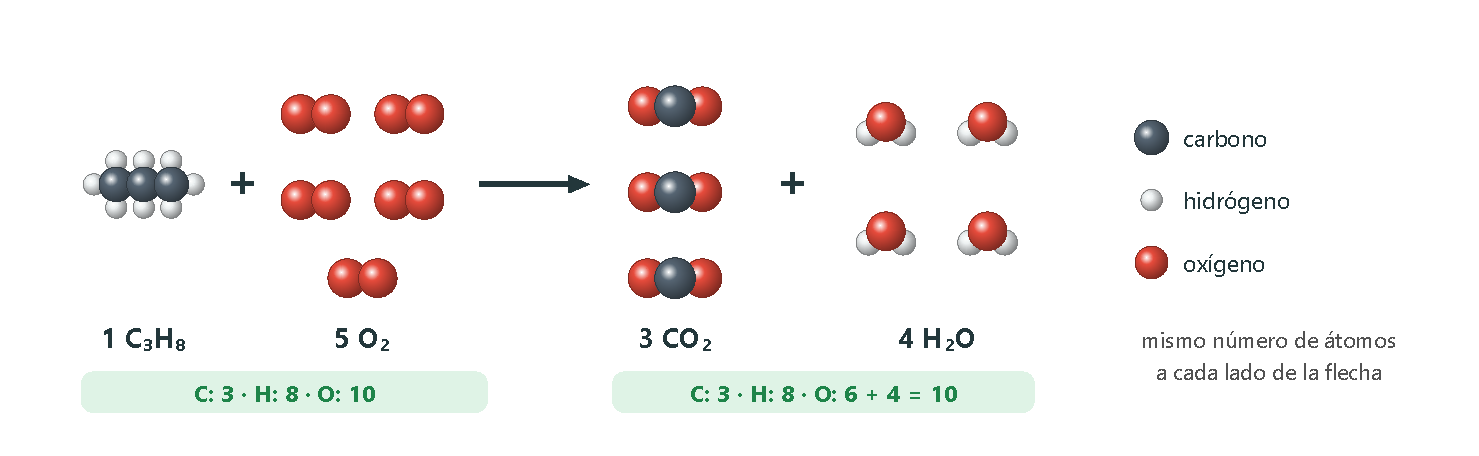
\includegraphics[width=0.9\textwidth]{images/UD6/ajuste_propano}
    \caption{Combustión del propano ajustada: a los dos lados hay 3 átomos de C, 8 de H y 10 de O.}
    \label{fig:ud6-propano}
\end{figure}

\begin{example}
    \textbf{Ajuste de la fotosíntesis.} Ajusta por tanteo la ecuación de la fotosíntesis:
    \ch{CO2 + H2O -> C6H12O6 + O2}.

    \textbf{Solución.} Carbono: 6 en la glucosa; ponemos un 6 delante del \ch{CO2}: \ch{6 CO2 + H2O -> C6H12O6 + O2}.
    Hidrógeno: 12 en la glucosa; ponemos un 6 delante del agua: \ch{6 CO2 + 6 H2O -> C6H12O6 + O2}. Oxígeno: a la izquierda hay
    \(6 \cdot 2 + 6 = 18\); a la derecha, 6 en la glucosa, así que faltan 12, es decir, 6 moléculas de \ch{O2}:
    \[ \ch{6 CO2 + 6 H2O -> C6H12O6 + 6 O2} \]
\end{example}

\begin{example}
    \textbf{Método algebraico.} Ajusta: \ch{NH3 + O2 -> NO + H2O}.

    \textbf{Solución.} \(a\,\ch{NH3} + b\,\ch{O2} \rightarrow c\,\ch{NO} + d\,\ch{H2O}\). N: \(a = c\); H: \(3a = 2d\); O: \(2b = c + d\). Con \(a = 1\):
    \(c = 1\), \(d = \frac{3}{2}\), \(b = \frac{5}{4}\). Multiplicamos todo por 4:
    \[ \ch{4 NH3 + 5 O2 -> 4 NO + 6 H2O} \]
\end{example}

\begin{exercise}
    Ajusta por tanteo estas reacciones: a) \ch{C5H12 + O2 -> CO2 + H2O}; b) \ch{SO2 + O2 -> SO3};
    c) \ch{HBr + Ca(OH)2 -> CaBr2 + H2O}; d) \ch{FeS2 + O2 -> Fe2O3 + SO2}; e) \ch{Ag2SO4 + KCl -> K2SO4 + AgCl};
    f) \ch{Mg + HCl -> MgCl2 + H2}; g) \ch{H3PO4 + KOH -> K3PO4 + H2O}.
    \begin{solu}
        a) \textcolor{red}{\ch{C5H12 + 8 O2 -> 5 CO2 + 6 H2O}}; b) \textcolor{red}{\ch{2 SO2 + O2 -> 2 SO3}};
        c) \textcolor{red}{\ch{2 HBr + Ca(OH)2 -> CaBr2 + 2 H2O}}; d) \textcolor{red}{\ch{4 FeS2 + 11 O2 -> 2 Fe2O3 + 8 SO2}};
        e) \textcolor{red}{\ch{Ag2SO4 + 2 KCl -> K2SO4 + 2 AgCl}}; f) \textcolor{red}{\ch{Mg + 2 HCl -> MgCl2 + H2}};
        g) \textcolor{red}{\ch{H3PO4 + 3 KOH -> K3PO4 + 3 H2O}}.
    \end{solu}
\end{exercise}

\begin{exercise}
    Ajusta por el método algebraico: a) la fermentación de la glucosa, \ch{C6H12O6 -> C2H5OH + CO2}; b) \ch{Cu + HNO3 ->
    Cu(NO3)2 + NO2 + H2O}.
    \begin{solu}
        a) \textcolor{blue}{C: \(6a = 2b + c\); H: \(12a = 6b\); O: \(6a = b + 2c\). Con \(a = 1\): \(b = 2\), \(c = 2\).}
        \textcolor{red}{\ch{C6H12O6 -> 2 C2H5OH + 2 CO2}}.
        b) \textcolor{blue}{\(a\,\ch{Cu} + b\,\ch{HNO3} \rightarrow c\,\ch{Cu(NO3)2} + d\,\ch{NO2} + e\,\ch{H2O}\). Cu: \(a = c\); H: \(b = 2e\); N: \(b = 2c + d\);
        O: \(3b = 6c + 2d + e\). Con \(a = c = 1\): \(b = 2 + d\) y \(3b = 6 + 2d + b/2\); resolviendo, \(b = 4\), \(d = 2\), \(e = 2\).}
        \textcolor{red}{\ch{Cu + 4 HNO3 -> Cu(NO3)2 + 2 NO2 + 2 H2O}}.
    \end{solu}
\end{exercise}

\begin{exercise}
    ¿Están ajustadas estas ecuaciones? Ajusta las que no lo estén: a) \ch{2 H2SO4 + S -> 3 SO2 + 2 H2O};
    b) \ch{2 HI + H2SO4 -> I2 + SO2 + 2 H2O}; c) \ch{2 KClO3 -> 2 KCl + 3 O2}; d) \ch{Fe2O3 + 2 CO -> 2 Fe + 2 CO2}.
    \begin{solu}
        \textcolor{red}{a), b) y c) están ajustadas.} d) \textcolor{blue}{Hay 5 O a la izquierda y 4 a la derecha.}
        \textcolor{red}{\ch{Fe2O3 + 3 CO -> 2 Fe + 3 CO2}}.
    \end{solu}
\end{exercise}

\subsection{Interpretación de la ecuación química}

Una vez ajustada, la ecuación da información cuantitativa: los coeficientes indican la proporción en que reaccionan y se forman
las sustancias, tanto en \textbf{moléculas} como en \textbf{moles} (al multiplicar todo por \(N_A\) la proporción no cambia) y,
si son gases en las mismas condiciones de presión y temperatura, en \textbf{volumen} (ley de Gay-Lussac). Con las masas molares,
la proporción en moles se convierte en proporción en \textbf{masa}.

\begin{table}[H]
    \centering
    \caption{Información de la ecuación ajustada de la combustión del propano}
    \vspace{-5pt}
    \begin{tabular}{@{}lcccc@{}}
        \toprule
        & \ch{C3H8(g)} & \ch{+ 5 O2(g)} & \ch{-> 3 CO2(g)} & \ch{+ 4 H2O(l)} \\
        \midrule
        Moléculas & 1 & 5 & 3 & 4 \\[3pt]
        Moles & 1 & 5 & 3 & 4 \\[3pt]
        Masa (g) & \(1 \cdot 44 = 44\) & \(5 \cdot 32 = 160\) & \(3 \cdot 44 = 132\) & \(4 \cdot 18 = 72\) \\[3pt]
        Volumen de gas (c.\,n.) & \qty{22.4}{\litre} & \qty{112}{\litre} & \qty{67.2}{\litre} & — (líquido) \\
        \bottomrule
    \end{tabular}
    \label{tab:ud6-interpretacion}
\end{table}

Fíjate en que la masa se conserva (\(44 + 160 = 132 + 72 = \qty{204}{\gram}\)), pero el número de moles no tiene por qué
conservarse (6 moles de reactivos dan 7 de productos).

\begin{example}
    \textbf{Leer una ecuación.} Ajusta e interpreta en moléculas, moles y gramos la reacción del hierro con el ácido clorhídrico:
    \ch{Fe(s) + HCl(aq) -> FeCl3(aq) + H2(g) ^}.

    \textbf{Solución.} Ajustada por tanteo: \ch{2 Fe(s) + 6 HCl(aq) -> 2 FeCl3(aq) + 3 H2(g) ^}.
    \begin{itemize}
        \item Dos átomos de hierro reaccionan con seis moléculas de \ch{HCl} para dar dos unidades de \ch{FeCl3} y tres moléculas
        de hidrógeno gaseoso, que se desprende.
        \item 2 mol de Fe reaccionan con 6 mol de \ch{HCl} y dan 2 mol de \ch{FeCl3} y 3 mol de \ch{H2}.
        \item Con las masas molares (Fe 55,8; \ch{HCl} 36,5; \ch{FeCl3} 162,3; \ch{H2} \qty{2}{\gram\per\mol}):
        \(\qty{111.6}{\gram}\) de Fe reaccionan con \qty{219}{\gram} de \ch{HCl} y dan \qty{324.6}{\gram} de \ch{FeCl3} y
        \qty{6}{\gram} de \ch{H2}. Se conserva la masa: \(\num{111.6} + 219 = \num{324.6} + 6 = \qty{330.6}{\gram}\).
    \end{itemize}
\end{example}

\begin{exercise}
    Ajusta y da toda la información cuantitativa (moles y gramos) de: a) \ch{Na + H2O -> NaOH + H2};
    b) \ch{Mg + H2SO4 -> MgSO4 + H2}; c) \ch{CH4 + O2 -> CO2 + H2O}.
    \begin{solu}
        a) \textcolor{red}{\ch{2 Na + 2 H2O -> 2 NaOH + H2}}: 2 mol (\qty{46}{\gram}) de Na y 2 mol (\qty{36}{\gram}) de agua dan
        2 mol (\qty{80}{\gram}) de \ch{NaOH} y 1 mol (\qty{2}{\gram}) de \ch{H2}; \(82 = 82\).
        b) \textcolor{red}{\ch{Mg + H2SO4 -> MgSO4 + H2}} (ya ajustada): \qty{24.3}{\gram} de Mg y \qty{98}{\gram} de ácido dan
        \qty{120.3}{\gram} de \ch{MgSO4} y \qty{2}{\gram} de \ch{H2}.
        c) \textcolor{red}{\ch{CH4 + 2 O2 -> CO2 + 2 H2O}}: \qty{16}{\gram} de metano y \qty{64}{\gram} de oxígeno dan
        \qty{44}{\gram} de \ch{CO2} y \qty{36}{\gram} de agua; \(80 = 80\).
    \end{solu}
\end{exercise}

\begin{exercise}
    En la reacción \ch{N2(g) + 3 H2(g) -> 2 NH3(g)}, ¿qué volumen de hidrógeno reacciona con \qty{12}{\litre} de nitrógeno?
    ¿Qué volumen de amoníaco se forma? Todos los gases están en las mismas condiciones.
    \begin{solu}
        \textcolor{blue}{En las mismas condiciones, la proporción en volumen es la de los coeficientes: 1 : 3 : 2.}
        \textcolor{red}{\qty{36}{\litre} de \ch{H2} y \qty{24}{\litre} de \ch{NH3}}.
    \end{solu}
\end{exercise}

%========================================================================================
\section{Tipos de reacciones químicas}\label{sec:ud6-tipos}
%========================================================================================

Las reacciones se pueden clasificar con muchos criterios: por su \textbf{velocidad} (rápidas o lentas), por la \textbf{energía}
que intercambian (exotérmicas o endotérmicas), por el \textbf{mecanismo} o por las \textbf{partículas que se transfieren}. Vamos a
estudiar estos dos últimos.

\subsection{Según el mecanismo de reacción}

\begin{figure}[H]
    \centering
    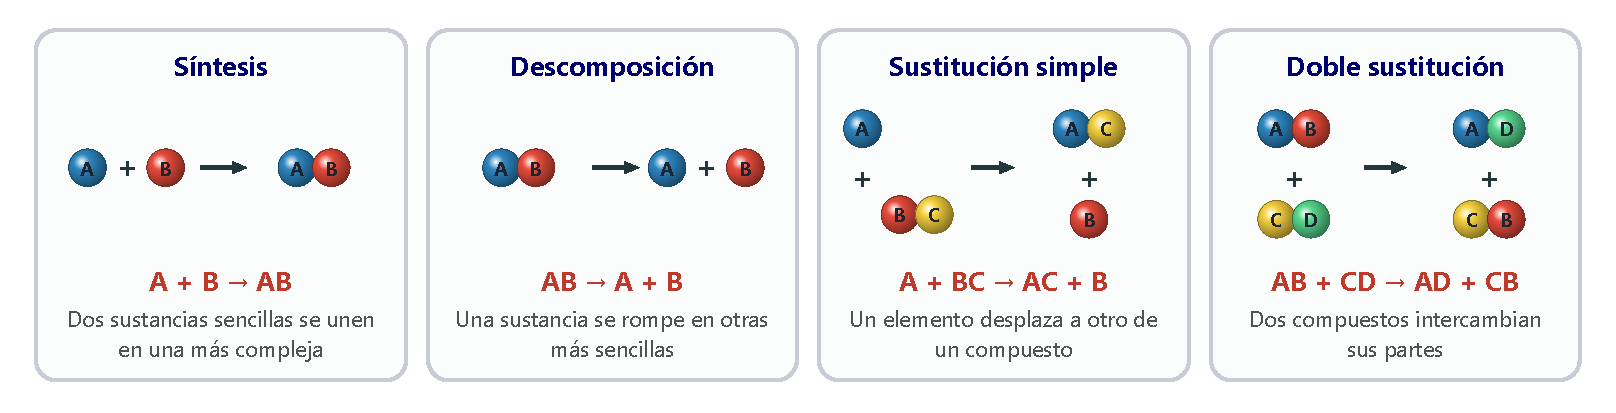
\includegraphics[width=\textwidth]{images/UD6/tipos_reaccion}
    \caption{Los cuatro tipos de reacción según su mecanismo.}
    \label{fig:ud6-tipos}
\end{figure}

\paragraph{Síntesis (\ch{A + B -> AB}).} Dos o más reactivos sencillos se combinan para dar un compuesto más complejo. Tienen un
gran interés industrial: así se obtienen medicamentos, plásticos o cosméticos. Por ejemplo, la síntesis del metanol, un
disolvente y combustible, \ch{CO(g) + 2 H2(g) -> CH3OH(g)}, o la del amoníaco, \ch{N2(g) + 3 H2(g) -> 2 NH3(g)}. Si se
obtiene un mol de compuesto a partir de sus elementos en su forma natural, se llama \textbf{reacción de formación}.

\paragraph{Descomposición (\ch{AB -> A + B}).} Una sustancia se rompe en otras más sencillas; es el proceso inverso de la
síntesis. El ácido carbónico de los refrescos se descompone en agua y \ch{CO2} (las burbujas), \ch{H2CO3(aq) -> H2O(l) + CO2(g)},
y el ácido nítrico se descompone con la luz, \ch{4 HNO3(l) -> 4 NO2(g) + O2(g) + 2 H2O(l)}; el \ch{NO2} es el gas pardo que da
color anaranjado al aire contaminado.

\paragraph{Sustitución o desplazamiento simple (\ch{A + BC -> AC + B}).} Un elemento sustituye a otro en un compuesto. Es el
caso de la \textbf{reacción termita}, \ch{2 Al + Fe2O3 -> Al2O3 + 2 Fe}, que desprende tanto calor que el hierro sale fundido;
se usa para soldar raíles.

\paragraph{Doble sustitución (\ch{AB + CD -> AD + CB}).} Dos compuestos intercambian sus partes. Al mezclar disoluciones de
nitrato de plomo(II) y de yoduro de potasio se forma yoduro de plomo(II), un sólido amarillo que precipita:
\ch{Pb(NO3)2(aq) + 2 KI(aq) -> PbI2(s) v + 2 KNO3(aq)}.

\begin{example}
    \textbf{Clasificar reacciones.} Clasifica según su mecanismo: a) \ch{2 Al + 3 S -> Al2S3};
    b) \ch{Ca(OH)2 -> CaO + H2O}; c) \ch{2 Li + 2 H2O -> 2 LiOH + H2}; d) \ch{BaCl2 + Na2SO4 -> BaSO4 + 2 NaCl}.

    \textbf{Solución.} a) \textbf{Síntesis}: dos elementos se unen en un compuesto. b) \textbf{Descomposición}: un compuesto da dos
    más sencillos. c) \textbf{Sustitución simple}: el litio desplaza a uno de los hidrógenos del agua. d) \textbf{Doble
    sustitución}: el bario y el sodio intercambian sus aniones.
\end{example}

\begin{exercise}
    Clasifica según su mecanismo: a) \ch{4 Al + 3 O2 -> 2 Al2O3}; b) \ch{CaCO3 -> CaO + CO2};
    c) \ch{Zn + CuSO4 -> ZnSO4 + Cu}; d) \ch{AgNO3 + NaCl -> AgCl + NaNO3}; e) \ch{2 H2O2 -> 2 H2O + O2};
    f) \ch{Cl2 + 2 KBr -> 2 KCl + Br2}.
    \begin{solu}
        \textcolor{red}{Síntesis: a). Descomposición: b) y e). Sustitución simple: c) y f). Doble sustitución: d).}
    \end{solu}
\end{exercise}

\subsection{Según las partículas que se transfieren}

\subsubsection{Reacciones ácido-base: transferencia de protones}

Según la teoría de \textbf{Brønsted y Lowry}:

\begin{definition}[Ácidos y bases]
    Un \textbf{ácido} es una sustancia capaz de \textbf{ceder protones} (\ch{H+}); en agua produce iones hidronio, \ch{H3O+}.

    Una \textbf{base} es una sustancia capaz de \textbf{captar protones}; en agua produce iones hidróxido, \ch{OH-}.
\end{definition}

El cloruro de hidrógeno se disocia por completo en agua, \ch{HCl + H2O -> H3O+ + Cl-}: es un \textbf{ácido fuerte}. El
amoníaco capta protones del agua, \ch{NH3 + H2O <=> NH4+ + OH-}, pero solo en pequeña proporción: es una \textbf{base débil}.

\begin{table}[H]
    \centering
    \caption{Propiedades de los ácidos y de las bases}
    \vspace{-5pt}
    \begin{tabular}{@{}L{6.6cm}L{6.6cm}@{}}
        \toprule
        \textbf{Ácidos} & \textbf{Bases} \\
        \midrule
        Sabor agrio (limón, vinagre) & Sabor amargo \\[3pt]
        Son corrosivos & Son cáusticos: pueden quemar la piel \\[3pt]
        Atacan a metales como Fe, Zn o Mg desprendiendo \ch{H2} & Tacto suave, jabonoso \\[3pt]
        Con la caliza (\ch{CaCO3}) desprenden \ch{CO2}: «prueba del ácido» de los geólogos & Neutralizan a los ácidos \\
        \bottomrule
    \end{tabular}
    \label{tab:ud6-acidos}
\end{table}

\paragraph{La escala de pH.} La acidez de una disolución depende de su concentración de \ch{H3O+}. Como esta concentración varía
mucho, se usa una escala logarítmica, el \textbf{pH}: \(\mathrm{pH} = -\log\,[\ch{H3O+}]\). El agua pura y las disoluciones
neutras tienen pH 7; las ácidas, menos de 7, y las básicas, más de 7. Cada unidad de pH supone una concentración de \ch{H3O+} diez
veces mayor o menor.

\begin{figure}[H]
    \centering
    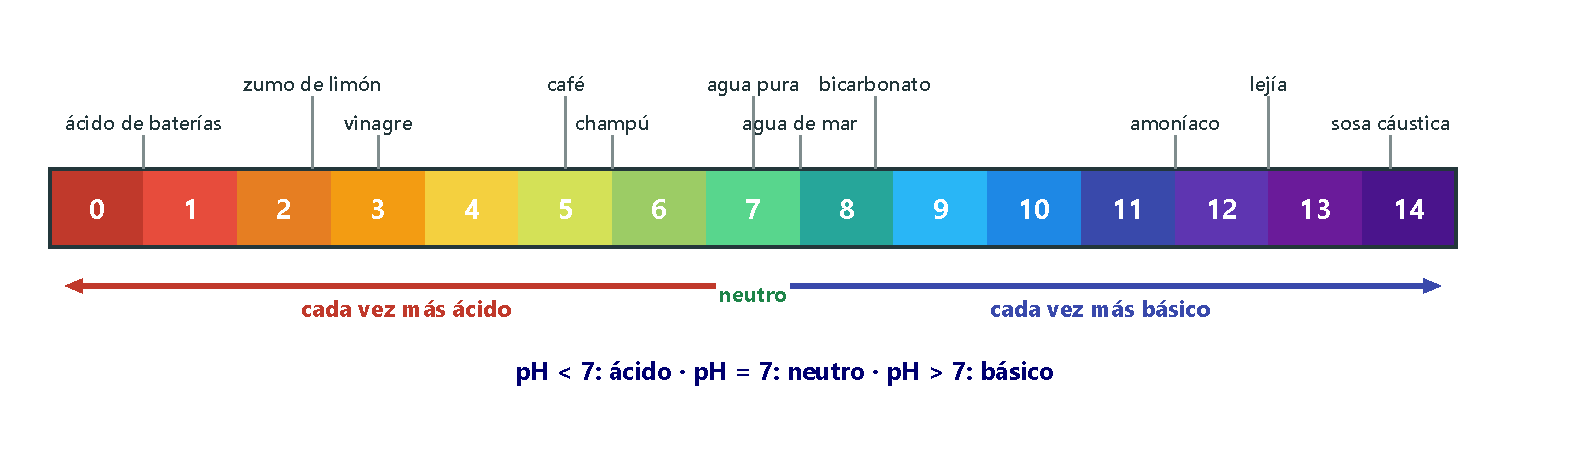
\includegraphics[width=0.9\textwidth]{images/UD6/escala_ph}
    \caption{Escala de pH de algunas sustancias de uso cotidiano.}
    \label{fig:ud6-ph}
\end{figure}

\paragraph{Reacciones de neutralización.} Cuando un ácido y una base reaccionan, el ácido transfiere protones a la base y se
forman una \textbf{sal} y \textbf{agua}; ambos pierden sus propiedades características: se \textbf{neutralizan}.
\[ \text{ácido} + \text{base} \ch{->} \text{sal} + \text{agua} \qquad\qquad \ch{HCl + NaOH -> NaCl + H2O} \]
Por ejemplo, los antiácidos (bicarbonato de sodio, hidróxido de magnesio) son bases que neutralizan el exceso de ácido clorhídrico
del estómago.

\begin{example}
    \textbf{Picaduras.} Las avispas inyectan con su picadura una sustancia básica y las hormigas, ácido fórmico. ¿Qué pondrías sobre
    cada picadura para aliviarla?

    \textbf{Solución.} Una sustancia de carácter contrario, que la neutralice: sobre la picadura de avispa, un ácido débil, como el
    vinagre o el zumo de limón; sobre la de hormiga, una base débil, como bicarbonato disuelto en agua o amoníaco diluido. En los dos
    casos se produce una neutralización: ácido + base \(\rightarrow\) sal + agua.
\end{example}

\begin{exercise}
    Completa y ajusta estas neutralizaciones: a) \ch{Al(OH)3 + HBr ->}; b) \ch{H2SO4 + KOH ->};
    c) \ch{Ca(OH)2 + HNO3 ->}; d) \ch{HCl + Fe(OH)3 ->}; e) \ch{NH3 + HCl ->}; f) \ch{CH3COOH + KOH ->}.
    \begin{solu}
        a) \textcolor{red}{\ch{Al(OH)3 + 3 HBr -> AlBr3 + 3 H2O}}; b) \textcolor{red}{\ch{H2SO4 + 2 KOH -> K2SO4 + 2 H2O}};
        c) \textcolor{red}{\ch{Ca(OH)2 + 2 HNO3 -> Ca(NO3)2 + 2 H2O}}; d) \textcolor{red}{\ch{3 HCl + Fe(OH)3 -> FeCl3 + 3 H2O}};
        e) \textcolor{red}{\ch{NH3 + HCl -> NH4Cl}} (el amoníaco capta el protón y no se forma agua);
        f) \textcolor{red}{\ch{CH3COOH + KOH -> CH3COOK + H2O}}.
    \end{solu}
\end{exercise}

\begin{exercise}
    a) El zumo de limón tiene pH 2 y el café, pH 5. ¿Cuántas veces mayor es la concentración de \ch{H3O+} en el limón? b) Escribe la
    reacción con la que un antiácido de hidróxido de magnesio neutraliza el ácido del estómago.
    \begin{solu}
        a) \textcolor{blue}{Tres unidades de pH equivalen a un factor \(10^3\).} \textcolor{red}{1000 veces mayor}.
        b) \textcolor{red}{\ch{Mg(OH)2 + 2 HCl -> MgCl2 + 2 H2O}}.
    \end{solu}
\end{exercise}

\subsubsection{Reacciones redox: transferencia de electrones}

\begin{definition}[Oxidación y reducción]
    En una reacción \textbf{redox} una sustancia \textbf{pierde electrones} y otra los \textbf{gana}.
    \begin{itemize}
        \item La sustancia que pierde electrones \textbf{se oxida}; es el \textbf{reductor}, porque reduce a la otra.
        \item La sustancia que gana electrones \textbf{se reduce}; es el \textbf{oxidante}.
    \end{itemize}
\end{definition}

En la oxidación del hierro por el oxígeno del aire, \ch{4 Fe + 3 O2 -> 2 Fe2O3}, cada proceso se puede escribir por separado
en una \textbf{semirreacción}:
\[ \text{oxidación: } \ch{Fe -> Fe^3+ + 3 e-} \qquad\qquad \text{reducción: } \ch{O2 + 4 e- -> 2 O^2-} \]
El Fe se oxida (es el reductor) y el \ch{O2} se reduce (es el oxidante). La oxidación y la reducción \textbf{ocurren siempre a la
vez}: los electrones que pierde una sustancia los gana la otra. Para obtener la ecuación global, se multiplica cada semirreacción
por un número de forma que los electrones perdidos y ganados sean los mismos (aquí, 12) y se suman: \(4 \cdot (\ch{Fe -> Fe^3+ +
3 e-})\) y \(3 \cdot (\ch{O2 + 4 e- -> 2 O^2-})\) dan \ch{4 Fe + 3 O2 -> 2 Fe2O3}.

Las reacciones redox están por todas partes: las \textbf{combustiones}, la respiración, la corrosión de los metales y su protección,
la \textbf{obtención de metales} a partir de sus minerales y el funcionamiento de \textbf{pilas y baterías}.

\begin{remark}
    \textbf{La pila Daniell.} Si el zinc y los iones \ch{Cu^2+} están en recipientes separados, \ch{Zn + CuSO4 -> ZnSO4 + Cu},
    los electrones que pierde el zinc tienen que viajar por un cable para llegar al cobre: se genera una \textbf{corriente
    eléctrica}. Así funciona una pila: una reacción redox convierte energía química en eléctrica.
\end{remark}

\begin{exercise}
    En estas reacciones redox, escribe las semirreacciones e indica el oxidante y el reductor: a) \ch{S + O2 -> SO2};
    b) \ch{2 Fe + 3 Cl2 -> 2 FeCl3}; c) \ch{Zn + 2 HCl -> ZnCl2 + H2}.
    \begin{solu}
        a) \textcolor{blue}{\ch{S -> S^4+ + 4 e-} (oxidación); \ch{O2 + 4 e- -> 2 O^2-} (reducción).} \textcolor{red}{Reductor: S;
        oxidante: \ch{O2}.} b) \textcolor{blue}{\ch{Fe -> Fe^3+ + 3 e-}; \ch{Cl2 + 2 e- -> 2 Cl-}.} \textcolor{red}{Reductor: Fe;
        oxidante: \ch{Cl2}.} c) \textcolor{blue}{\ch{Zn -> Zn^2+ + 2 e-}; \ch{2 H+ + 2 e- -> H2}.} \textcolor{red}{Reductor: Zn;
        oxidante: \ch{H+} (del \ch{HCl}).}
    \end{solu}
\end{exercise}

\subsubsection{Reacciones de precipitación: transferencia de iones}

En estas reacciones, iones presentes en una \textbf{disolución acuosa} se combinan y forman una \textbf{sustancia insoluble}, el
\textbf{precipitado}, que enturbia el líquido y acaba depositándose en el fondo. Por ejemplo, al mezclar nitrato de plata y
cromato de sodio se forma cromato de plata, rojo e insoluble:
\[ \ch{2 AgNO3(aq) + Na2CrO4(aq) -> Ag2CrO4(s) v + 2 NaNO3(aq)} \]
Este precipitado se usa en el \textbf{método de Golgi} para teñir las neuronas y poder verlas al microscopio.

Las reacciones de precipitación sirven para \textbf{eliminar metales} de las aguas residuales, para \textbf{analizar} qué iones
contiene una muestra o, en inmunología, en las pruebas serológicas, en las que un antígeno y sus anticuerpos forman un precipitado.
Otras veces son indeseadas: el \ch{CaCO3} que precipita en las tuberías (la cal) las obstruye y estropea calentadores y
electrodomésticos.

\begin{example}
    \textbf{Doble clasificación.} Ajusta y clasifica según su mecanismo y según la partícula transferida:
    a) \ch{K2SO4 + CaBr2 -> KBr + CaSO4 v}; b) \ch{HgO -> Hg + O2}.

    \textbf{Solución.} a) \ch{K2SO4 + CaBr2 -> 2 KBr + CaSO4 v}. Es una \textbf{doble sustitución} y, como el \ch{CaSO4} es poco
    soluble y precipita, una reacción de \textbf{precipitación}.

    b) \ch{2 HgO -> 2 Hg + O2}. Es una \textbf{descomposición} y una reacción \textbf{redox}: el mercurio gana electrones (se
    reduce) y el oxígeno los pierde (se oxida):
    \[ 2 \cdot (\ch{Hg^2+ + 2 e- -> Hg}) \qquad\quad \ch{2 O^2- -> O2 + 4 e-} \]
\end{example}

\begin{exercise}
    Ajusta y clasifica estas reacciones según los dos criterios que hemos visto: a) \ch{Cu(NO3)2 -> CuO + NO2 + O2};
    b) \ch{K2CO3 + CaCl2 -> KCl + CaCO3 v}; c) \ch{Fe + Cl2 -> FeCl3}.
    \begin{solu}
        a) \textcolor{red}{\ch{2 Cu(NO3)2 -> 2 CuO + 4 NO2 + O2}}: descomposición y redox (el N se reduce y parte del O se oxida).
        b) \textcolor{red}{\ch{K2CO3 + CaCl2 -> 2 KCl + CaCO3 v}}: doble sustitución y precipitación.
        c) \textcolor{red}{\ch{2 Fe + 3 Cl2 -> 2 FeCl3}}: síntesis y redox (el Fe se oxida y el \ch{Cl2} se reduce).
    \end{solu}
\end{exercise}

%========================================================================================
\section{Cálculos estequiométricos}\label{sec:ud6-estequiometria}
%========================================================================================

En el laboratorio, en la industria y hasta en la cocina es necesario saber qué cantidad de cada sustancia hace falta o se obtiene en
un proceso. Si una receta de bizcocho para 8 personas lleva 4 huevos y \qty{200}{\gram} de harina, para 4 personas necesitarás la
mitad de todo: la receta fija una proporción. En química, esa proporción la dan los coeficientes de la ecuación ajustada.

\begin{definition}[Cálculos estequiométricos]
    Son los cálculos que permiten conocer las cantidades de reactivos y productos que intervienen en una reacción a partir de su
    \textbf{ecuación ajustada}.
\end{definition}

Para resolver un problema de estequiometría, identifica primero el \textbf{dato} y la \textbf{incógnita} y sigue el esquema de la
figura~\ref{fig:ud6-esquema}. El paso clave, común a todos los problemas, es el 3: la relación entre moles que dan los coeficientes.

\begin{figure}[H]
    \centering
    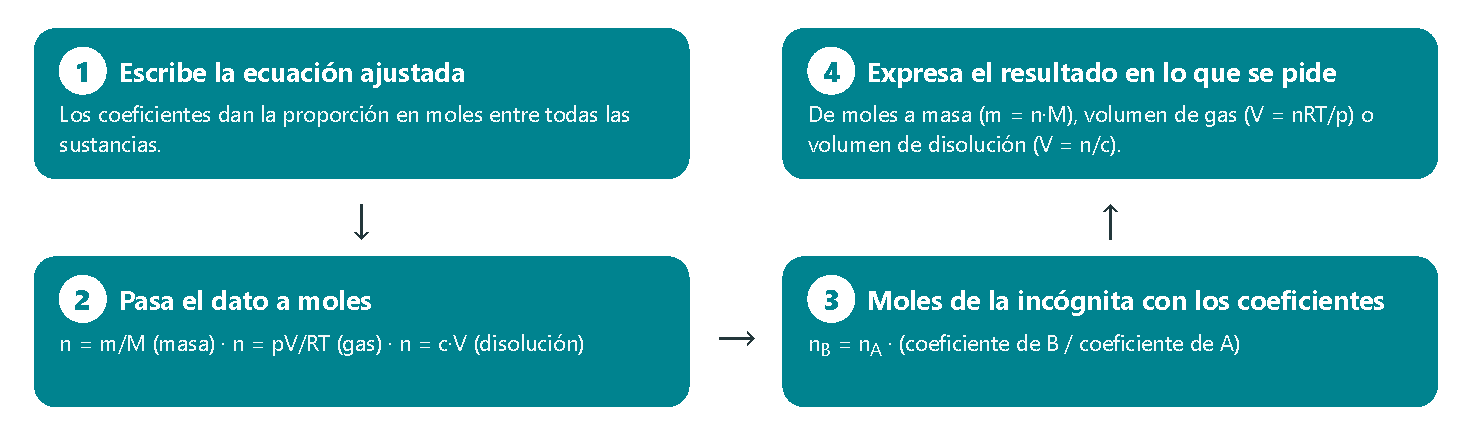
\includegraphics[width=0.85\textwidth]{images/UD6/esquema_estequiometria}
    \caption{Pasos para resolver un problema de estequiometría.}
    \label{fig:ud6-esquema}
\end{figure}

\begin{example}
    \textbf{Factor de conversión o proporción.} El agua oxigenada se descompone en agua y oxígeno:
    \ch{H2O2(aq) -> H2O(l) + 1/2 O2(g)}. ¿Cuánto oxígeno se desprende al descomponerse \qty{3}{\mol} de agua oxigenada? ¿Qué
    masa es?

    \textbf{Solución.} Dato: \qty{3}{\mol} de \ch{H2O2}; incógnita: el \ch{O2}. Por cada mol de \ch{H2O2} se forma \(\frac{1}{2}\) mol
    de \ch{O2}. Podemos usar un \textbf{factor de conversión}:
    \[ \qty{3}{\mol}\ \ch{H2O2} \cdot \frac{\frac{1}{2}\ \unit{\mol}\ \ch{O2}}{\qty{1}{\mol}\ \ch{H2O2}} = \qty{1.5}{\mol}\ \ch{O2} \]
    o una \textbf{proporción}: \(\dfrac{1}{1/2} = \dfrac{3}{x} \Rightarrow x = \qty{1.5}{\mol}\). Su masa es
    \(m = n \cdot M = \num{1.5} \cdot 32 = \qty{48}{\gram}\) de \ch{O2}.
\end{example}

\subsection{Cálculos con masas y volúmenes de gases}

En los pasos 2 y 4 hay que pasar de masa o volumen a moles y al revés. Recuerda:
\begin{itemize}
    \item \textbf{Masa}: \(n = \dfrac{m}{M}\). Si es un sólido o un líquido del que conocemos el volumen, primero se calcula la masa
    con la densidad, \(m = d \cdot V\).
    \item \textbf{Gases}: \(n = \dfrac{p\,V}{R\,T}\), con \(R = \qty{0.082}{\atm\litre\per\mol\per\kelvin}\). En
    \textbf{condiciones normales} (c.\,n.: \qty{0}{\degreeCelsius} y \qty{1}{\atm}), un mol de cualquier gas ocupa
    \qty{22.4}{\litre}. Recuerda también que \(\qty{1}{\atm} = \qty{1.013e5}{\pascal} = \qty{760}{\mmHg}\).
    \item Si los reactivos y productos son \textbf{gases en las mismas condiciones} de presión y temperatura, los coeficientes dan
    directamente la proporción entre sus volúmenes.
\end{itemize}

\begin{example}
    \textbf{De masa a volumen de gas.} Se hacen reaccionar \qty{20.0}{\gram} de zinc con ácido clorhídrico en exceso:
    \ch{Zn + 2 HCl -> ZnCl2 + H2 ^}. ¿Qué volumen de hidrógeno se obtiene a \qty{25}{\degreeCelsius} y \qty{740}{\mmHg}?

    \textbf{Solución.} \textbf{1.} La ecuación ya está ajustada. \textbf{2.} Moles de Zn: \(n = \dfrac{\qty{20.0}{\gram}}{\qty{65.4}{\gram\per\mol}} =
    \qty{0.306}{\mol}\). \textbf{3.} Por cada mol de Zn se forma 1 mol de \ch{H2}:
    \[ \qty{0.306}{\mol}\ \ch{Zn} \cdot \frac{\qty{1}{\mol}\ \ch{H2}}{\qty{1}{\mol}\ \ch{Zn}} = \qty{0.306}{\mol}\ \ch{H2} \]
    \textbf{4.} Con \(p = \dfrac{740}{760} = \qty{0.974}{\atm}\) y \(T = 25 + 273 = \qty{298}{\kelvin}\):
    \[ V = \frac{n R T}{p} = \frac{\num{0.306} \cdot \num{0.082} \cdot 298}{\num{0.974}} = \qty{7.67}{\litre}\ \text{de}\ \ch{H2} \]
\end{example}

\begin{example}
    \textbf{De volumen de gas a masa.} Con la misma reacción, ¿qué masa de \ch{HCl} hace falta para obtener \qty{15}{\litre} de
    \ch{H2} medidos en condiciones normales?

    \textbf{Solución.} Encadenamos los factores de conversión, partiendo siempre del dato:
    \[ \qty{15}{\litre}\ \ch{H2} \cdot \frac{\qty{1}{\mol}\ \ch{H2}}{\qty{22.4}{\litre}\ \ch{H2}} \cdot
    \frac{\qty{2}{\mol}\ \ch{HCl}}{\qty{1}{\mol}\ \ch{H2}} \cdot \frac{\qty{36.5}{\gram}\ \ch{HCl}}{\qty{1}{\mol}\ \ch{HCl}} =
    \qty{48.9}{\gram}\ \ch{HCl} \]
\end{example}

\begin{exercise}
    Calcula el volumen de \ch{CO2}, medido a \qty{5}{\degreeCelsius} y \qty{600}{\mmHg}, que se produce al quemar \qty{50}{\gram}
    de butano, \ch{C4H10}.
    \begin{solu}
        \textcolor{blue}{\ch{2 C4H10 + 13 O2 -> 8 CO2 + 10 H2O}; \(n(\ch{C4H10}) = 50/58 = \qty{0.862}{\mol}\);
        \(n(\ch{CO2}) = 4 \cdot \num{0.862} = \qty{3.45}{\mol}\); \(p = 600/760 = \qty{0.789}{\atm}\).}
        \(V = \dfrac{\num{3.45} \cdot \num{0.082} \cdot 278}{\num{0.789}} = \textcolor{red}{\qty{99.6}{\litre}}\).
    \end{solu}
\end{exercise}

\begin{exercise}
    Se hacen reaccionar \qty{8.0}{\gram} de ácido sulfúrico con zinc en exceso, y se obtienen sulfato de zinc e hidrógeno.
    a) Escribe y ajusta la reacción. b) ¿Qué masa de hidrógeno se forma? c) ¿Qué volumen ocupa a \qty{27}{\degreeCelsius} y
    \qty{720}{\mmHg}?
    \begin{solu}
        a) \textcolor{red}{\ch{Zn + H2SO4 -> ZnSO4 + H2}}. b) \textcolor{blue}{\(n(\ch{H2SO4}) = 8/98 = \qty{0.0816}{\mol} = n(\ch{H2})\).}
        \(m = \num{0.0816} \cdot 2 = \textcolor{red}{\qty{0.163}{\gram}}\). c) \(V = \dfrac{\num{0.0816} \cdot \num{0.082} \cdot 300}{720/760}
        = \textcolor{red}{\qty{2.12}{\litre}}\).
    \end{solu}
\end{exercise}

\begin{exercise}
    Con la reacción del ejercicio anterior, ¿qué masa de zinc se necesita para obtener \qty{30}{\litre} de hidrógeno en condiciones
    normales?
    \begin{solu}
        \(\dfrac{30}{\num{22.4}} = \qty{1.34}{\mol}\) de \ch{H2} \(=\) mol de Zn; \(m = \num{1.34} \cdot \num{65.4} =
        \textcolor{red}{\qty{87.6}{\gram}}\) de Zn.
    \end{solu}
\end{exercise}

\subsection{Cálculos con disoluciones}

Muchas reacciones, en el laboratorio, en la industria y en los seres vivos, tienen lugar en \textbf{disolución acuosa}. Hay que
recordar que la sustancia que reacciona es el \textbf{soluto}; el disolvente, en general, no interviene. En los pasos 2 y 4 se
relaciona la cantidad de soluto con la concentración (unidad 2):
\[ \%\,\text{masa} = \frac{m_{\text{soluto}}}{m_{\text{disolución}}} \cdot 100 \qquad
c = \frac{n_{\text{soluto}}}{V_{\text{disolución}}} \qquad \gamma = \frac{m_{\text{soluto}}}{V_{\text{disolución}}} \]
A veces, sin embargo, el agua es también reactivo o producto: lee con atención el enunciado.

\begin{example}
    \textbf{Neutralización.} El hidróxido de magnesio reacciona con el ácido clorhídrico para dar cloruro de magnesio y agua.
    a) ¿Qué masa de ácido clorhídrico del 36\,\% en masa se necesita para neutralizar \qty{120}{\gram} de \ch{Mg(OH)2}?
    b) ¿Qué volumen se necesitaría si se usara ácido clorhídrico \qty{1.5}{\mol\per\litre}?

    \textbf{Solución.} \ch{Mg(OH)2 + 2 HCl -> MgCl2 + 2 H2O}; \(M(\ch{Mg(OH)2}) = \qty{58.3}{\gram\per\mol}\);
    \(M(\ch{HCl}) = \qty{36.5}{\gram\per\mol}\).

    a) \[ \qty{120}{\gram}\ \ch{Mg(OH)2} \cdot \frac{\qty{1}{\mol}}{\qty{58.3}{\gram}} \cdot \frac{\qty{2}{\mol}\ \ch{HCl}}{\qty{1}{\mol}\ \ch{Mg(OH)2}}
    = \qty{4.12}{\mol}\ \ch{HCl} \ \rightarrow\ \num{4.12} \cdot \num{36.5} = \qty{150.3}{\gram}\ \ch{HCl} \]
    Como el ácido solo tiene un 36\,\% de \ch{HCl}: \(\qty{150.3}{\gram}\ \ch{HCl} \cdot \dfrac{\qty{100}{\gram}\ \text{dis.}}{\qty{36}{\gram}\ \ch{HCl}} =
    \qty{417}{\gram}\) de disolución.

    b) \(V = \dfrac{n}{c} = \dfrac{\qty{4.12}{\mol}}{\qty{1.5}{\mol\per\litre}} = \qty{2.74}{\litre}\).
\end{example}

\begin{remark}
    \textbf{Volumetrías.} Una \textbf{valoración} o volumetría es una técnica de análisis para conocer la concentración de una
    disolución. Se añade gota a gota, con una bureta, una disolución de concentración conocida hasta que la reacción termina, lo que
    se detecta con un \textbf{indicador} que cambia de color. Con el volumen gastado y la estequiometría se calcula la concentración
    desconocida (figura~\ref{fig:ud6-valoracion}).
\end{remark}

\begin{figure}[H]
    \centering
    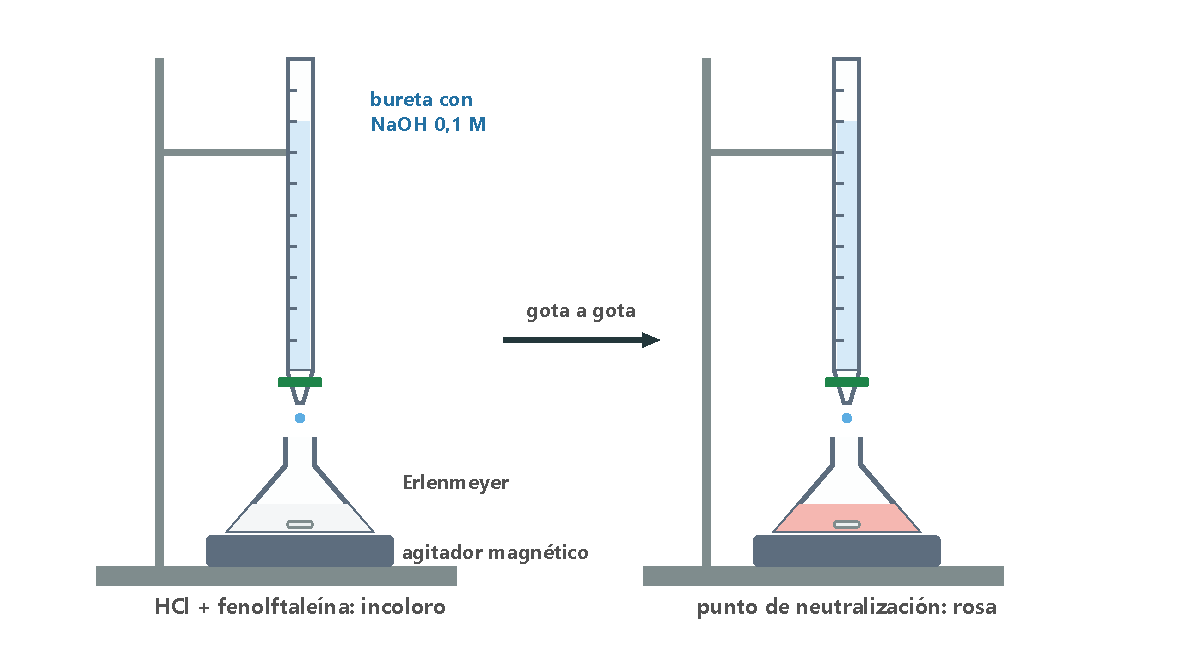
\includegraphics[width=0.62\textwidth]{images/UD6/valoracion}
    \caption{Valoración de un ácido con una base: la fenolftaleína se vuelve rosa al completarse la neutralización.}
    \label{fig:ud6-valoracion}
\end{figure}

\begin{exercise}
    Calcula el volumen de ácido clorhídrico \qty{0.5}{\mol\per\litre} necesario para neutralizar \qty{400}{\mL} de una disolución
    de hidróxido de calcio \qty{0.2}{\mol\per\litre}.
    \begin{solu}
        \textcolor{blue}{\ch{Ca(OH)2 + 2 HCl -> CaCl2 + 2 H2O}; \(n(\ch{Ca(OH)2}) = \num{0.4} \cdot \num{0.2} = \qty{0.08}{\mol}\);
        \(n(\ch{HCl}) = \qty{0.16}{\mol}\).} \(V = \num{0.16}/\num{0.5} = \textcolor{red}{\qty{0.32}{\litre} = \qty{320}{\mL}}\).
    \end{solu}
\end{exercise}

\begin{exercise}
    El nitrato de plata reacciona con el cloruro de sodio y precipita cloruro de plata. a) Escribe y ajusta la reacción. b) ¿Qué
    volumen de \ch{AgNO3} \qty{0.5}{\mol\per\litre} reacciona con \qty{200}{\mL} de \ch{NaCl} \qty{1.2}{\mol\per\litre}? c) ¿Qué
    masa de precipitado se obtiene?
    \begin{solu}
        a) \textcolor{red}{\ch{AgNO3 + NaCl -> AgCl v + NaNO3}}. b) \textcolor{blue}{\(n(\ch{NaCl}) = \num{0.2} \cdot \num{1.2} =
        \qty{0.24}{\mol} = n(\ch{AgNO3})\).} \(V = \num{0.24}/\num{0.5} = \textcolor{red}{\qty{480}{\mL}}\).
        c) \(\num{0.24} \cdot \num{143.4} = \textcolor{red}{\qty{34.4}{\gram}}\) de \ch{AgCl}.
    \end{solu}
\end{exercise}

\subsection{Reactivo limitante}

Los coeficientes de la ecuación ajustada dan la proporción \textbf{fija} en que se combinan los reactivos. Si las cantidades que
mezclamos no guardan esa proporción, la reacción se detiene cuando se acaba uno de ellos y del otro sobra una parte
(figura~\ref{fig:ud6-limitante}).

\begin{definition}[Reactivo limitante]
    Es el reactivo que \textbf{se agota primero} y, por tanto, el que determina la cantidad de productos que se forma. El que no se
    agota es el \textbf{reactivo en exceso}. Cuál es cada uno depende de las cantidades iniciales.
\end{definition}

\begin{figure}[H]
    \centering
    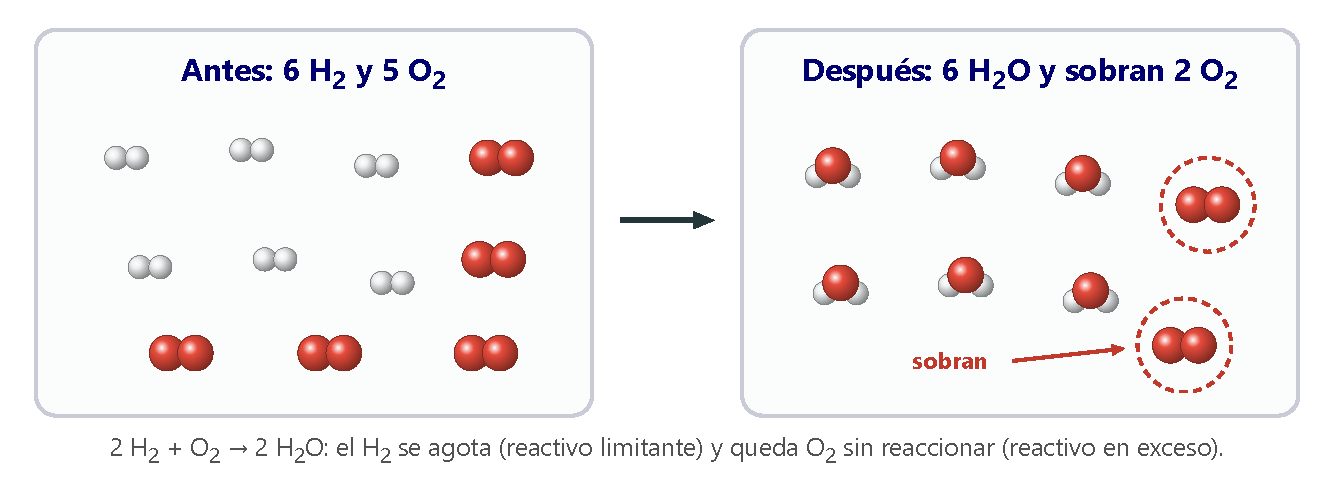
\includegraphics[width=0.8\textwidth]{images/UD6/reactivo_limitante}
    \caption{Con 6 moléculas de \ch{H2} y 5 de \ch{O2} solo se forman 6 de agua: el hidrógeno es el reactivo limitante.}
    \label{fig:ud6-limitante}
\end{figure}

Para una reacción \(a\,\ch{A} + b\,\ch{B} \rightarrow c\,\ch{C}\), hay dos formas de encontrar el reactivo limitante:
\begin{itemize}
    \item \textbf{Método 1.} Calcula los moles iniciales, \(n_A\) y \(n_B\). Con los coeficientes, calcula los moles de B que
    reaccionarían con todo A: \(n_B' = n_A \cdot \frac{b}{a}\). Si hay menos B de lo necesario (\(n_B < n_B'\)), \textbf{B es el
    limitante}; si hay más (\(n_B > n_B'\)), \textbf{A es el limitante}.
    \item \textbf{Método 2.} Calcula cuánto producto se obtendría si reaccionase todo A (\(n_A \cdot \frac{c}{a}\)) y si reaccionase
    todo B (\(n_B \cdot \frac{c}{b}\)). El limitante es el que da \textbf{menos} producto.
\end{itemize}
A partir de ese momento, todos los cálculos se hacen con la cantidad del reactivo limitante.

\begin{example}
    \textbf{Tricloruro de aluminio.} En un recipiente se introducen \qty{4}{\mol} de aluminio y \qty{5}{\mol} de cloro, que
    reaccionan para dar \ch{AlCl3}. a) ¿Cuál es el reactivo limitante? b) ¿Cuánto sobra del otro? c) ¿Cuántos moles de \ch{AlCl3} se
    forman?

    \textbf{Solución.} \ch{2 Al + 3 Cl2 -> 2 AlCl3}.

    a) Cloro necesario para que reaccione todo el aluminio: \(\qty{4}{\mol}\ \ch{Al} \cdot \dfrac{\qty{3}{\mol}\ \ch{Cl2}}{\qty{2}{\mol}\ \ch{Al}} =
    \qty{6}{\mol}\ \ch{Cl2}\). Solo hay 5: \textbf{el cloro es el limitante} y el aluminio está en exceso.

    b) Aluminio que reacciona: \(\qty{5}{\mol}\ \ch{Cl2} \cdot \dfrac{2}{3} = \qty{3.33}{\mol}\); sobran \(4 - \num{3.33} = \qty{0.67}{\mol}\) de Al.

    c) Con el limitante: \(\qty{5}{\mol}\ \ch{Cl2} \cdot \dfrac{2}{3} = \qty{3.33}{\mol}\) de \ch{AlCl3}.
\end{example}

\begin{example}
    \textbf{Con masas.} Se mezclan \qty{20}{\gram} de hidrógeno y \qty{64}{\gram} de oxígeno y se hace saltar una chispa:
    \ch{2 H2 + O2 -> 2 H2O}. ¿Qué masa de agua se forma? ¿Qué sobra?

    \textbf{Solución.} \(n(\ch{H2}) = 20/2 = \qty{10}{\mol}\); \(n(\ch{O2}) = 64/32 = \qty{2}{\mol}\). Para \qty{2}{\mol} de \ch{O2}
    hacen falta \qty{4}{\mol} de \ch{H2}, y hay 10: \textbf{el oxígeno es el limitante}. Se forman \(2 \cdot 2 = \qty{4}{\mol}\) de
    agua, es decir, \(4 \cdot 18 = \qty{72}{\gram}\), y sobran \(10 - 4 = \qty{6}{\mol}\) de \ch{H2} (\qty{12}{\gram}). Comprobamos:
    \(20 + 64 = 72 + 12\).
\end{example}

\begin{exercise}
    El cobre reacciona con el ácido nítrico concentrado: \ch{Cu + 4 HNO3 -> Cu(NO3)2 + 2 NO2 + 2 H2O}. Se hacen reaccionar
    \qty{2.5}{\gram} de cobre con \qty{20}{\mL} de ácido nítrico \qty{3}{\mol\per\litre}. ¿Qué volumen de \ch{NO2} se obtiene,
    medido a \qty{20}{\degreeCelsius} y \qty{1.2}{\atm}?
    \begin{solu}
        \textcolor{blue}{\(n(\ch{Cu}) = \num{2.5}/\num{63.5} = \qty{0.0394}{\mol}\), que necesitarían \(4 \cdot \num{0.0394} =
        \qty{0.158}{\mol}\) de \ch{HNO3}; solo hay \(\num{0.02} \cdot 3 = \qty{0.06}{\mol}\): el \ch{HNO3} es el limitante.
        \(n(\ch{NO2}) = \num{0.06}/2 = \qty{0.03}{\mol}\).} \(V = \dfrac{\num{0.03} \cdot \num{0.082} \cdot 293}{\num{1.2}} =
        \textcolor{red}{\qty{0.60}{\litre}}\).
    \end{solu}
\end{exercise}

\begin{exercise}
    El acetileno, \ch{C2H2}, se usa en los sopletes de soldadura: \ch{2 C2H2 + 5 O2 -> 4 CO2 + 2 H2O}. Si se queman
    \qty{10}{\mol} de \ch{C2H2} con \qty{20}{\mol} de \ch{O2}, ¿cuál es el limitante? ¿Qué volumen de \ch{CO2} se forma a
    \qty{1800}{\degreeCelsius} y \qty{6}{\atm}?
    \begin{solu}
        \textcolor{blue}{Para \qty{10}{\mol} de \ch{C2H2} harían falta \qty{25}{\mol} de \ch{O2}: el \ch{O2} es el limitante.}
        \textcolor{red}{Limitante: \ch{O2}}. \(n(\ch{CO2}) = 20 \cdot \frac{4}{5} = \qty{16}{\mol}\);
        \(V = \dfrac{16 \cdot \num{0.082} \cdot 2073}{6} = \textcolor{red}{\qty{453}{\litre}}\).
    \end{solu}
\end{exercise}

\subsection{Rendimiento de una reacción}

En la práctica casi nunca se obtiene toda la cantidad de producto que predice la estequiometría: hay reacciones secundarias que
dan otros productos, la reacción no llega a completarse, las condiciones no son las ideales o se pierde algo de producto al
manipularlo. En la industria, que fabrica productos por toneladas, una mejora pequeña del rendimiento supone un gran ahorro.

\begin{definition}[Rendimiento]
    Es el cociente entre la cantidad de producto que se obtiene realmente y la que se obtendría en teoría, expresado en tanto por
    ciento:
    \[ \text{rendimiento}\ (\%) = \frac{\text{cantidad real de producto}}{\text{cantidad teórica de producto}} \cdot 100 \]
    Las dos cantidades deben estar en la misma magnitud (masa, moles o volumen en las mismas condiciones).
\end{definition}

\begin{example}
    \textbf{Descomposición del bicarbonato.} Al calentar hidrogenocarbonato de sodio se obtienen carbonato de sodio, agua y
    \ch{CO2}. Si se calientan \qty{20}{\gram} de \ch{NaHCO3} y el rendimiento es del 80\,\%, ¿qué masa de \ch{Na2CO3} se obtiene?

    \textbf{Solución.} La reacción es
    \[ \ch{2 NaHCO3(s) -> Na2CO3(s) + H2O(g) + CO2(g)} \]
    con \(M(\ch{NaHCO3}) = \qty{84}{\gram\per\mol}\) y \(M(\ch{Na2CO3}) = \qty{106}{\gram\per\mol}\). Masa teórica:
    \[ \qty{20}{\gram}\ \ch{NaHCO3} \cdot \frac{\qty{1}{\mol}}{\qty{84}{\gram}} \cdot \frac{\qty{1}{\mol}\ \ch{Na2CO3}}{\qty{2}{\mol}\ \ch{NaHCO3}}
    \cdot \frac{\qty{106}{\gram}}{\qty{1}{\mol}} = \qty{12.6}{\gram} \]
    Masa real: \(\num{12.6} \cdot \dfrac{80}{100} = \qty{10.1}{\gram}\) de \ch{Na2CO3}.
\end{example}

\begin{exercise}
    El nitrato de amonio, un fertilizante, se obtiene así: \ch{NH3 + HNO3 -> NH4NO3}. ¿Qué masa se obtiene al mezclar
    \qty{100}{\gram} de \ch{NH3} con \qty{40}{\gram} de \ch{HNO3} si el rendimiento es del 70\,\%?
    \begin{solu}
        \textcolor{blue}{\(n(\ch{NH3}) = 100/17 = \qty{5.88}{\mol}\); \(n(\ch{HNO3}) = 40/63 = \qty{0.635}{\mol}\): el \ch{HNO3} es el
        limitante. Teórico: \(\num{0.635} \cdot 80 = \qty{50.8}{\gram}\).} Real: \(\num{50.8} \cdot \num{0.70} =
        \textcolor{red}{\qty{35.6}{\gram}}\) de \ch{NH4NO3}.
    \end{solu}
\end{exercise}

\begin{exercise}
    El nitruro de silicio, \ch{Si3N4}, es un material cerámico muy duro y resistente al calor. Si \qty{28}{\gram} de silicio
    reaccionan con nitrógeno en exceso y se obtienen \qty{42}{\gram} de \ch{Si3N4}, ¿cuál es el rendimiento?
    \begin{solu}
        \textcolor{blue}{\ch{3 Si + 2 N2 -> Si3N4}; \(n(\ch{Si}) = 28/\num{28.1} = \qty{0.996}{\mol}\); \(n(\ch{Si3N4}) = \qty{0.332}{\mol}\);
        masa teórica \(\num{0.332} \cdot \num{140.3} = \qty{46.6}{\gram}\).} Rendimiento \(= \dfrac{42}{\num{46.6}} \cdot 100 =
        \textcolor{red}{\qty{90}{\percent}}\).
    \end{solu}
\end{exercise}

\subsection{Riqueza o pureza de los reactivos}

Los reactivos que se usan en la industria, y muchos minerales, contienen \textbf{impurezas} mezcladas con la sustancia de interés.

\begin{definition}[Riqueza]
    Es el porcentaje en masa de sustancia pura que contiene una muestra:
    \[ \text{riqueza}\ (\%) = \frac{\text{masa de sustancia pura}}{\text{masa total de la muestra}} \cdot 100 \]
    En los cálculos estequiométricos solo interviene la sustancia pura.
\end{definition}

Un método de análisis consiste en hacer reaccionar la muestra y medir la cantidad de producto: la estequiometría dice cuánta
sustancia pura había.

\begin{example}
    \textbf{Riqueza de una caliza.} La caliza es una roca formada sobre todo por carbonato de calcio, que reacciona con el ácido
    clorhídrico: \ch{CaCO3(s) + 2 HCl(aq) -> CaCl2(aq) + H2O(l) + CO2(g) ^}. Se ponen sobre una balanza un vaso con ácido en
    exceso y \qty{250}{\gram} de caliza. Al terminar la reacción, la balanza marca \qty{99}{\gram} menos, la masa del \ch{CO2} que
    se ha escapado. ¿Cuál es la riqueza de la caliza?

    \textbf{Solución.}
    \[ \qty{99}{\gram}\ \ch{CO2} \cdot \frac{\qty{1}{\mol}\ \ch{CO2}}{\qty{44}{\gram}} \cdot \frac{\qty{1}{\mol}\ \ch{CaCO3}}{\qty{1}{\mol}\ \ch{CO2}}
    \cdot \frac{\qty{100}{\gram}\ \ch{CaCO3}}{\qty{1}{\mol}} = \qty{225}{\gram}\ \ch{CaCO3} \]
    \[ \text{riqueza} = \frac{225}{250} \cdot 100 = \qty{90}{\percent} \]
\end{example}

\begin{exercise}
    La calcopirita, \ch{CuFeS2}, es un mineral del que se extrae el cobre. Al tostarla: \ch{2 CuFeS2 + 5 O2 -> 2 Cu + 2 FeO + 4
    SO2}. Si se tuestan \qty{150}{\gram} de mineral con un 70\,\% de \ch{CuFeS2} y el rendimiento es del 80\,\%, ¿qué masa de
    cobre se obtiene? ¿Y si el rendimiento fuera del 100\,\%?
    \begin{solu}
        \textcolor{blue}{Masa pura: \(150 \cdot \num{0.70} = \qty{105}{\gram}\); \(M(\ch{CuFeS2}) = \qty{183.3}{\gram\per\mol}\);
        \(n = \qty{0.573}{\mol}\) de \ch{CuFeS2} \(=\) mol de Cu.} Con rendimiento del 100\,\%: \(\num{0.573} \cdot \num{63.5} =
        \textcolor{red}{\qty{36.4}{\gram}}\); con el 80\,\%: \textcolor{red}{\qty{29.1}{\gram}} de Cu.
    \end{solu}
\end{exercise}

\begin{exercise}
    Se mezclan \qty{25}{\mL} de hidróxido de sodio \qty{2}{\mol\per\litre} con \qty{30}{\mL} de ácido fluorhídrico
    \qty{2.5}{\mol\per\litre} y se obtienen fluoruro de sodio y agua. a) Escribe y ajusta la reacción. b) ¿Cuál es el reactivo
    limitante? c) ¿Qué masa de \ch{NaF} se obtiene? d) ¿Y si el rendimiento es del 75\,\%?
    \begin{solu}
        a) \textcolor{red}{\ch{NaOH + HF -> NaF + H2O}}. b) \textcolor{blue}{\(n(\ch{NaOH}) = \qty{0.05}{\mol}\);
        \(n(\ch{HF}) = \qty{0.075}{\mol}\).} \textcolor{red}{Limitante: \ch{NaOH}}; sobran \qty{0.025}{\mol} de \ch{HF}.
        c) \(\num{0.05} \cdot 42 = \textcolor{red}{\qty{2.1}{\gram}}\). d) \textcolor{red}{\qty{1.6}{\gram}} de \ch{NaF}.
    \end{solu}
\end{exercise}

%========================================================================================
\section{La energía en las reacciones químicas}\label{sec:ud6-energia}
%========================================================================================

En una reacción se rompen enlaces de los reactivos, lo que requiere \textbf{aportar} energía, y se forman enlaces nuevos en los
productos, lo que \textbf{desprende} energía. El balance de las dos cosas hace que las reacciones químicas vayan siempre
acompañadas de un intercambio de energía con el entorno, casi siempre en forma de calor.

\subsection{Calor de reacción y entalpía}

\begin{definition}[Calor de reacción]
    Es la energía, en forma de calor, \(Q\), que intercambia con su entorno un sistema en el que se produce una reacción química.
    \begin{itemize}
        \item Si se desprende más energía al formar los enlaces de la que se gasta en romperlos, la reacción desprende calor: es
        \textbf{exotérmica} (\(Q < 0\)). Las combustiones son exotérmicas.
        \item Si cuesta más romper los enlaces de lo que se recupera al formar los nuevos, la reacción absorbe calor: es
        \textbf{endotérmica} (\(Q > 0\)). Cocinar un alimento es un ejemplo cotidiano de proceso endotérmico.
    \end{itemize}
\end{definition}

La mayoría de las reacciones que estudiaremos tienen lugar a \textbf{presión constante} (en recipientes abiertos a la atmósfera).
En ese caso, el calor de reacción coincide con la variación de una magnitud llamada \textbf{entalpía}, \(H\):
\[ Q_p = \Delta H = \sum H_{\text{productos}} - \sum H_{\text{reactivos}} \]
La entalpía es una \textbf{función de estado}: su variación solo depende de los estados inicial y final, no del camino seguido. Es,
además, una magnitud \textbf{extensiva}: depende de la cantidad de sustancia.

\begin{figure}[H]
    \centering
    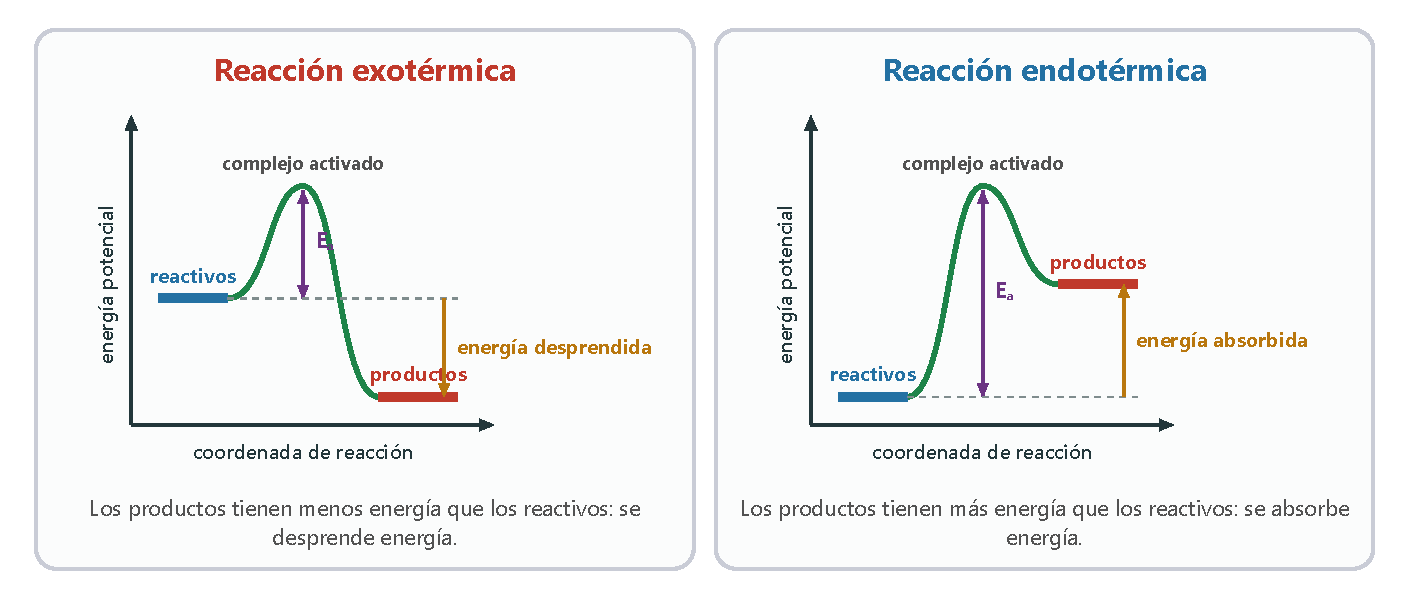
\includegraphics[width=0.85\textwidth]{images/UD6/exo_endo}
    \caption{Diagramas entálpicos de una reacción exotérmica (\(\Delta H < 0\)) y de una endotérmica (\(\Delta H > 0\)).}
    \label{fig:ud6-exo-endo}
\end{figure}

Los \textbf{diagramas entálpicos} (figura~\ref{fig:ud6-exo-endo}) representan la energía del sistema a medida que avanza la
reacción. Fíjate en que todas las reacciones, también las exotérmicas, necesitan un aporte inicial de energía, la \textbf{energía
de activación}, para empezar: por eso hay que encender una vela con una cerilla, aunque después la combustión se mantenga sola.

Algunos productos aprovechan estos intercambios: las \textbf{bolsas de frío instantáneo} contienen una sal, como el nitrato de
amonio, cuya disolución en agua es endotérmica, y los \textbf{envases autocalentables} usan la reacción exotérmica del óxido de
calcio con el agua, \ch{CaO(s) + H2O(l) -> Ca(OH)2(s)}.

\subsection{Ecuaciones termoquímicas}

\begin{definition}[Ecuación termoquímica]
    Es una ecuación química ajustada que incluye el \textbf{estado físico} de todas las sustancias y la \textbf{variación de
    entalpía} de la reacción. Por ejemplo:
    \[ \ch{2 H2(g) + O2(g) -> 2 H2O(g)} \qquad \Delta H = \qty{-483.6}{\kilo\joule} \]
    indica que en la formación de 2 mol de vapor de agua se desprenden \qty{483.6}{\kilo\joule}.
\end{definition}

De ella se deduce que:
\begin{itemize}
    \item El proceso inverso es endotérmico y absorbe la misma energía: \ch{2 H2O(g) -> 2 H2(g) + O2(g)},
    \(\Delta H = \qty{+483.6}{\kilo\joule}\).
    \item Como la entalpía es extensiva, al formar 1 mol de \ch{H2O(g)} se desprende la mitad, \qty{241.8}{\kilo\joule}: si se
    multiplica la ecuación por un número, \(\Delta H\) se multiplica por el mismo número. Por eso en las ecuaciones termoquímicas
    se admiten coeficientes fraccionarios.
    \item \(\Delta H\) depende del estado físico (no es lo mismo formar agua líquida que vapor) y de la presión y la temperatura. Se
    llama \textbf{entalpía estándar}, \(\Delta H^\circ\), la de una reacción a \qty{1}{\bar} (aproximadamente \qty{1}{\atm}) y,
    normalmente, \qty{25}{\degreeCelsius}.
\end{itemize}

\begin{exercise}
    Con la ecuación termoquímica anterior, ¿qué energía se desprende al quemar \qty{10}{\gram} de hidrógeno para dar vapor de agua?
    \begin{solu}
        \textcolor{blue}{\(n(\ch{H2}) = 10/2 = \qty{5}{\mol}\); por cada 2 mol se desprenden \qty{483.6}{\kilo\joule}.}
        \(5 \cdot \dfrac{\num{483.6}}{2} = \textcolor{red}{\qty{1209}{\kilo\joule}}\) desprendidos.
    \end{solu}
\end{exercise}

\subsection{Medida experimental de la entalpía: el calorímetro}

Para medir el calor de reacción se lleva a cabo la reacción dentro de un \textbf{calorímetro}: un recipiente aislado que contiene
una masa conocida de agua (figura~\ref{fig:ud6-calorimetro}). Como sus paredes no dejan pasar el calor, todo el que desprende o
absorbe la reacción lo gana o lo pierde el agua, cuya temperatura cambia. Midiendo esa variación de temperatura:
\[ \Delta H = Q_p = -Q_{\text{agua}} = -m_{\text{agua}} \cdot c_{\text{agua}} \cdot \Delta T \qquad
c_{\text{agua}} = \qty{4.18}{\joule\per\gram\per\degreeCelsius} \]
Para medidas precisas hay que tener en cuenta también el calor que absorben las piezas del calorímetro.

\begin{figure}[H]
    \centering
    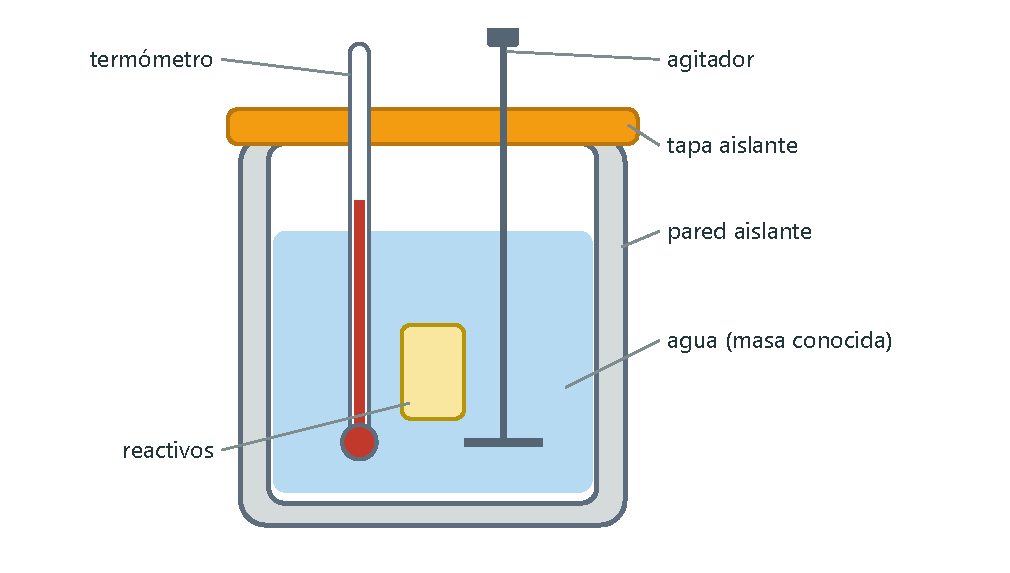
\includegraphics[width=0.5\textwidth]{images/UD6/calorimetro}
    \caption{Calorímetro: el calor de la reacción se mide por la variación de temperatura del agua.}
    \label{fig:ud6-calorimetro}
\end{figure}

\begin{exercise}
    En un calorímetro se mezclan \qty{100}{\mL} de \ch{HCl} \qty{1}{\mol\per\litre} con \qty{100}{\mL} de \ch{NaOH}
    \qty{1}{\mol\per\litre}, y la temperatura sube \qty{6.7}{\degreeCelsius}. Calcula la entalpía de neutralización por mol de
    agua formada. Supón que la mezcla tiene la densidad y el calor específico del agua.
    \begin{solu}
        \textcolor{blue}{\(Q_{\text{agua}} = 200 \cdot \num{4.18} \cdot \num{6.7} = \qty{5601}{\joule}\); se forman
        \(\num{0.1}\) mol de agua.} \(\Delta H = -\dfrac{\qty{5.60}{\kilo\joule}}{\qty{0.1}{\mol}} =
        \textcolor{red}{\qty{-56.0}{\kilo\joule\per\mol}}\).
    \end{solu}
\end{exercise}

\subsection{Ley de Hess}

Hay reacciones cuya entalpía no se puede medir directamente. Como la entalpía es una función de estado, se puede calcular
combinando otras reacciones conocidas:

\begin{definition}[Ley de Hess]
    La variación de entalpía de una reacción es la misma tanto si se produce en una sola etapa como en varias. Si una ecuación se
    puede obtener sumando otras (multiplicadas o invertidas si hace falta), su \(\Delta H\) se obtiene haciendo las mismas
    operaciones con sus entalpías.
\end{definition}

Por ejemplo, la combustión del carbono da el mismo calor si se produce directamente o pasando por monóxido de carbono
(figura~\ref{fig:ud6-hess}): \(\num{-110.5} + (\num{-283.0}) = \qty{-393.5}{\kilo\joule}\).

\begin{figure}[H]
    \centering
    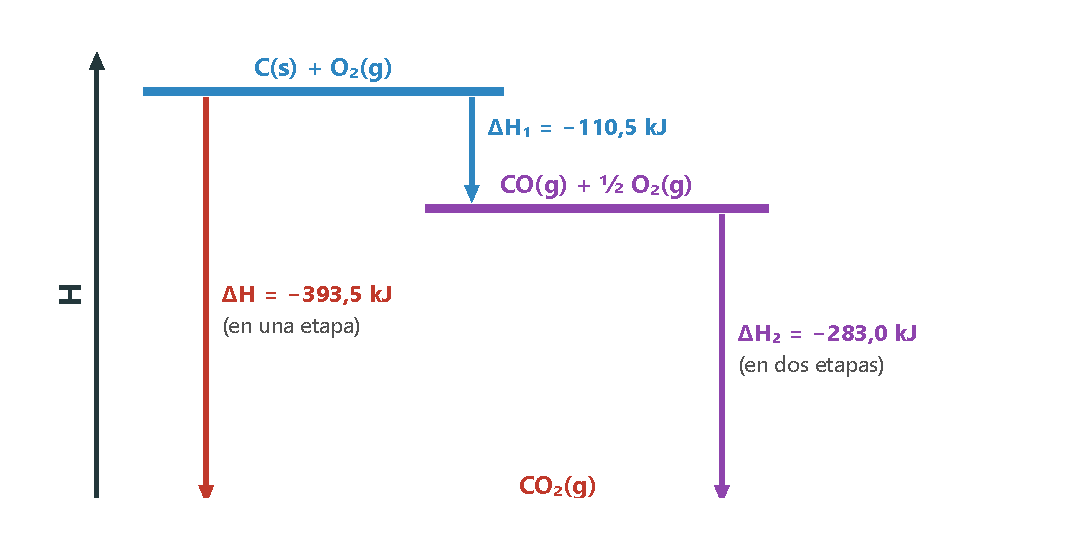
\includegraphics[width=0.6\textwidth]{images/UD6/hess}
    \caption{Ley de Hess: la entalpía de combustión del carbono no depende del camino.}
    \label{fig:ud6-hess}
\end{figure}

\begin{example}
    \textbf{Entalpía de formación del acetileno.} Con estos datos, calcula \(\Delta H\) para \ch{2 C(grafito) + H2(g) ->
    C2H2(g)}:
    \[ \begin{aligned}
        &\text{(A)}\ \ \ch{C(grafito) + O2(g) -> CO2(g)} && \Delta H_A = \qty{-393.5}{\kilo\joule} \\
        &\text{(B)}\ \ \ch{H2(g) + 1/2 O2(g) -> H2O(l)} && \Delta H_B = \qty{-285.8}{\kilo\joule} \\
        &\text{(C)}\ \ \ch{2 C2H2(g) + 5 O2(g) -> 4 CO2(g) + 2 H2O(l)} && \Delta H_C = \qty{-2599.2}{\kilo\joule}
    \end{aligned} \]

    \textbf{Solución.} Necesitamos 2 C a la izquierda (multiplicamos A por 2), 1 \ch{H2} a la izquierda (B tal cual) y 1 \ch{C2H2} a
    la derecha (invertimos C y la dividimos entre 2):
    \[ \begin{aligned}
        &\ch{2 C(grafito) + 2 O2 -> 2 CO2} && 2 \cdot (\num{-393.5}) = \qty{-787.0}{\kilo\joule} \\
        &\ch{H2 + 1/2 O2 -> H2O} && \qty{-285.8}{\kilo\joule} \\
        &\ch{2 CO2 + H2O -> C2H2 + 5/2 O2} && -\tfrac{1}{2} \cdot (\num{-2599.2}) = \qty{+1299.6}{\kilo\joule}
    \end{aligned} \]
    Al sumar, se cancelan el \ch{CO2}, el \ch{H2O} y el \ch{O2}: \ch{2 C(grafito) + H2 -> C2H2},
    \(\Delta H = -787{,}0 - 285{,}8 + 1299{,}6 = \qty{226.8}{\kilo\joule}\). Es endotérmica.
\end{example}

\begin{exercise}
    Con las entalpías de combustión del C(grafito) (\qty{-393.5}{\kilo\joule\per\mol}), del \ch{H2(g)}
    (\qty{-285.8}{\kilo\joule\per\mol}, dando agua líquida) y del \ch{CH4(g)} (\qty{-890.3}{\kilo\joule\per\mol}), calcula la
    entalpía de la reacción \ch{C(grafito) + 2 H2(g) -> CH4(g)}.
    \begin{solu}
        \textcolor{blue}{(A) + 2\(\cdot\)(B) \(-\) (C): \(\Delta H = -393{,}5 + 2 \cdot (-285{,}8) + 890{,}3\).}
        \(\Delta H = \textcolor{red}{\qty{-74.8}{\kilo\joule}}\).
    \end{solu}
\end{exercise}

\begin{exercise}
    Calcula la entalpía de oxidación del zinc, \ch{Zn(s) + 1/2 O2(g) -> ZnO(s)}, a partir de:
    \ch{Zn(s) + H2SO4(aq) -> ZnSO4(aq) + H2(g)}, \(\Delta H_A = \qty{-335}{\kilo\joule}\);
    \ch{2 H2(g) + O2(g) -> 2 H2O(l)}, \(\Delta H_B = \qty{-571.6}{\kilo\joule}\);
    \ch{ZnO(s) + H2SO4(aq) -> ZnSO4(aq) + H2O(l)}, \(\Delta H_C = \qty{-215}{\kilo\joule}\).
    \begin{solu}
        \textcolor{blue}{A + \(\frac{1}{2}\)B \(-\) C: \(\Delta H = -335 + \frac{1}{2}(-571{,}6) - (-215)\).}
        \(\Delta H = \textcolor{red}{\qty{-405.8}{\kilo\joule}}\).
    \end{solu}
\end{exercise}

\subsection{Entalpía de formación}

La entalpía de una reacción depende del estado físico de reactivos y productos. Por convenio, se toma como \textbf{estado estándar}
de una sustancia su forma más estable a \qty{1}{\bar} y \qty{25}{\degreeCelsius}.

\begin{definition}[Entalpía estándar de formación]
    La entalpía estándar de formación de un compuesto, \(\Delta H_f^\circ\), es la variación de entalpía de la reacción en la que se
    forma \textbf{un mol} del compuesto, en estado estándar, a partir de sus \textbf{elementos} en estado estándar. Por convenio, la
    de los elementos en su forma más estable (\ch{O2(g)}, \ch{N2(g)}, C(grafito), Fe(s), Hg(l)…) es \textbf{cero}.
\end{definition}

Aplicando la ley de Hess, la entalpía estándar de cualquier reacción se calcula a partir de las entalpías de formación tabuladas:
\[ \Delta H^\circ = \sum n_p\, \Delta H_f^\circ(\text{productos}) - \sum n_r\, \Delta H_f^\circ(\text{reactivos}) \]
donde \(n_p\) y \(n_r\) son los coeficientes de la ecuación ajustada: hacen falta porque los valores de la tabla son por mol.

\begin{table}[H]
    \centering
    \caption{Entalpías estándar de formación a \qty{25}{\degreeCelsius}}
    \vspace{-5pt}
    \begin{tabular}{@{}lr@{\hspace{1.5cm}}lr@{\hspace{1.5cm}}lr@{}}
        \toprule
        \textbf{Sustancia} & \makecell{\(\Delta H_f^\circ\)\\(\unit{\kilo\joule\per\mol})} &
        \textbf{Sustancia} & \makecell{\(\Delta H_f^\circ\)\\(\unit{\kilo\joule\per\mol})} &
        \textbf{Sustancia} & \makecell{\(\Delta H_f^\circ\)\\(\unit{\kilo\joule\per\mol})} \\
        \midrule
        \ch{H2O(g)} & \(-241{,}8\) & \ch{NO(g)} & \(90{,}3\) & \ch{CH4(g)} & \(-74{,}8\) \\[3pt]
        \ch{H2O(l)} & \(-285{,}8\) & \ch{NO2(g)} & \(33{,}2\) & \ch{C2H2(g)} & \(226{,}7\) \\[3pt]
        \ch{CO(g)} & \(-110{,}5\) & \ch{NH3(g)} & \(-46{,}2\) & \ch{C3H8(g)} & \(-103{,}8\) \\[3pt]
        \ch{CO2(g)} & \(-393{,}5\) & \ch{HCl(g)} & \(-92{,}3\) & \ch{C2H5OH(l)} & \(-277{,}7\) \\[3pt]
        \ch{SO2(g)} & \(-296{,}8\) & \ch{H2S(g)} & \(-20{,}6\) & \ch{CaCO3(s)} & \(-1206{,}9\) \\[3pt]
        \ch{SO3(g)} & \(-395{,}7\) & \ch{HNO3(l)} & \(-174{,}1\) & \ch{CaO(s)} & \(-635{,}1\) \\
        \bottomrule
    \end{tabular}
    \label{tab:ud6-formacion}
\end{table}

\begin{example}
    \textbf{Combustión del metano.} Con la tabla~\ref{tab:ud6-formacion}, calcula la entalpía de combustión del metano para dar
    \ch{CO2(g)} y \ch{H2O(l)}.

    \textbf{Solución.} \ch{CH4(g) + 2 O2(g) -> CO2(g) + 2 H2O(l)}.
    \[ \Delta H^\circ = \big[(-393{,}5) + 2 \cdot (-285{,}8)\big] - \big[(-74{,}8) + 2 \cdot 0\big] = \qty{-890.3}{\kilo\joule} \]
\end{example}

\begin{exercise}
    Calcula, con la tabla~\ref{tab:ud6-formacion}, la entalpía de combustión del etanol, \ch{C2H5OH(l)}, para dar \ch{CO2(g)} y
    \ch{H2O(l)}.
    \begin{solu}
        \textcolor{blue}{\ch{C2H5OH + 3 O2 -> 2 CO2 + 3 H2O}; \(\Delta H^\circ = 2(-393{,}5) + 3(-285{,}8) - (-277{,}7)\).}
        \(\Delta H^\circ = \textcolor{red}{\qty{-1366.7}{\kilo\joule\per\mol}}\).
    \end{solu}
\end{exercise}

\begin{exercise}
    Calcula la entalpía de combustión del acetileno, \ch{C2H2(g)}, con agua líquida como producto. ¿Qué energía se desprende al
    quemar \qty{1}{\kilo\gram} de acetileno?
    \begin{solu}
        \textcolor{blue}{\ch{C2H2 + 5/2 O2 -> 2 CO2 + H2O}; \(\Delta H^\circ = 2(-393{,}5) + (-285{,}8) - 226{,}7\).}
        \(\Delta H^\circ = \textcolor{red}{\qty{-1299.5}{\kilo\joule\per\mol}}\); \(n = 1000/26 = \qty{38.5}{\mol}\):
        \textcolor{red}{\qty{5.0e4}{\kilo\joule}} desprendidos.
    \end{solu}
\end{exercise}

\subsection{Entalpía de combustión}

\begin{definition}[Entalpía estándar de combustión]
    Es la variación de entalpía, \(\Delta H_c^\circ\), de la reacción en la que \textbf{un mol} de una sustancia reacciona
    completamente con oxígeno, con reactivos y productos en estado estándar.
\end{definition}

Es siempre negativa y mide el poder energético de un combustible. Con la ley de Hess, igual que con las de formación, se pueden
calcular entalpías de reacción a partir de entalpías de combustión tabuladas (fíjate en que la fórmula se invierte):
\[ \Delta H^\circ = \sum n_r\, \Delta H_c^\circ(\text{reactivos}) - \sum n_p\, \Delta H_c^\circ(\text{productos}) \]

\subsection{Entalpía de enlace}

\begin{definition}[Entalpía de enlace]
    Es la energía necesaria para romper un mol de enlaces entre dos átomos de una sustancia en estado gaseoso. Siempre es positiva.
\end{definition}

La entalpía de una reacción es, de forma aproximada, la diferencia entre la energía que se invierte en romper los enlaces de los
reactivos y la que se desprende al formar los de los productos:
\[ \Delta H^\circ \approx \sum \Delta H_{\text{enlaces rotos}} - \sum \Delta H_{\text{enlaces formados}} \]
El resultado es aproximado porque los valores tabulados son medias de los de muchas sustancias.

\begin{table}[H]
    \centering
    \caption{Entalpías medias de enlace (\unit{\kilo\joule\per\mol})}
    \vspace{-5pt}
    \begin{tabular}{@{}lr@{\hspace{1.2cm}}lr@{\hspace{1.2cm}}lr@{\hspace{1.2cm}}lr@{}}
        \toprule
        \textbf{Enlace} & \textbf{\(\Delta H\)} & \textbf{Enlace} & \textbf{\(\Delta H\)} & \textbf{Enlace} &
        \textbf{\(\Delta H\)} & \textbf{Enlace} & \textbf{\(\Delta H\)} \\
        \midrule
        H--H & 436 & C--H & 414 & C--C & 347 & N\(\equiv\)N & 945 \\[3pt]
        Cl--Cl & 243 & C--Cl & 339 & C=C & 614 & N--H & 391 \\[3pt]
        Br--Br & 193 & H--Cl & 432 & C=O & 745 & O=O & 498 \\[3pt]
        I--I & 151 & H--Br & 366 & C--O & 358 & O--H & 463 \\
        \bottomrule
    \end{tabular}
    \label{tab:ud6-enlace}
\end{table}

\begin{example}
    \textbf{Bromuro de hidrógeno.} Calcula la entalpía de formación del bromuro de hidrógeno gaseoso a partir de las entalpías de
    enlace.

    \textbf{Solución.} \ch{H2(g) + Br2(g) -> 2 HBr(g)}. Se rompen un enlace H--H y uno Br--Br, y se forman dos H--Br:
    \[ \Delta H = (436 + 193) - 2 \cdot 366 = \qty{-103}{\kilo\joule} \]
    Esto corresponde a 2 mol de \ch{HBr}: \(\Delta H_f \approx \qty{-51.5}{\kilo\joule\per\mol}\).
\end{example}

\begin{exercise}
    Calcula con las entalpías de enlace: a) la entalpía de formación del \ch{HCl(g)}; b) la entalpía de la reacción
    \ch{CH4(g) + Cl2(g) -> CH3Cl(g) + HCl(g)}.
    \begin{solu}
        a) \textcolor{blue}{\ch{H2 + Cl2 -> 2 HCl}: \(436 + 243 - 2 \cdot 432 = \qty{-185}{\kilo\joule}\) por 2 mol.}
        \textcolor{red}{\(\Delta H_f \approx \qty{-92.5}{\kilo\joule\per\mol}\)} (el valor tabulado es \(-92{,}3\)).
        b) \textcolor{blue}{Se rompen un C--H y un Cl--Cl; se forman un C--Cl y un H--Cl.} \(\Delta H = (414 + 243) - (339 + 432) =
        \textcolor{red}{\qty{-114}{\kilo\joule}}\).
    \end{solu}
\end{exercise}

%========================================================================================
\section{Combustiones}\label{sec:ud6-combustiones}
%========================================================================================

Las \textbf{combustiones} son reacciones redox en las que una sustancia, el \textbf{combustible}, reacciona con otra, el
\textbf{comburente} (normalmente el oxígeno del aire), desprendiendo energía. Su velocidad es muy variada: desde las lentísimas,
como la respiración celular, que «quema» la glucosa, hasta las explosiones.

\paragraph{Combustibles fósiles.} Alrededor del 80\,\% de la energía que consume la humanidad para cocinar, calentarse, moverse o
producir electricidad procede de quemar \textbf{combustibles fósiles}: el \textbf{petróleo}, el \textbf{carbón} y el \textbf{gas
natural}. Se formaron hace millones de años por la descomposición de restos de seres vivos. Contienen sobre todo
\textbf{hidrocarburos}, que arden según:
\[ \text{hidrocarburo} + \text{oxígeno} \ch{->} \text{dióxido de carbono} + \text{agua} + \text{energía} \]
Por ejemplo, el metano del gas natural: \ch{CH4(g) + 2 O2(g) -> CO2(g) + 2 H2O(l)}, \(\Delta H = \qty{-890}{\kilo\joule}\).

Son baratos y relativamente fáciles de extraer, transportar y almacenar, pero su uso tiene graves inconvenientes:
\begin{itemize}
    \item El \ch{CO2} que se emite al quemarlos \textbf{intensifica el efecto invernadero} y provoca un calentamiento global con
    consecuencias como el deshielo de los polos, la subida del nivel del mar, los fenómenos meteorológicos extremos, la
    desertificación, los incendios, la pérdida de biodiversidad o las migraciones forzadas.
    \item Sus impurezas producen al quemarse \textbf{óxidos de azufre y de nitrógeno}, que con el agua de la atmósfera forman ácidos
    sulfúrico y nítrico: es la \textbf{lluvia ácida}, que daña la vegetación, acidifica suelos y acuíferos y corroe edificios y
    estructuras metálicas.
    \item Sus reservas son \textbf{limitadas}, generan \textbf{dependencia} de los países productores y su control es fuente de
    conflictos y tensiones geopolíticas: son \textbf{recursos estratégicos}.
\end{itemize}

\paragraph{El hidrógeno verde.} Una alternativa es el hidrógeno, cuya combustión solo produce agua:
\ch{2 H2(g) + O2(g) -> 2 H2O(l)}, \(\Delta H = \qty{-571.6}{\kilo\joule}\). El hidrógeno no se encuentra libre en la
naturaleza; puede obtenerse por \textbf{electrólisis} del agua, el proceso inverso, que necesita energía eléctrica. Si esa energía
procede de fuentes renovables, se habla de \textbf{hidrógeno verde}: es una forma de \textbf{almacenar} la energía del sol o del
viento para usarla después, por ejemplo en pilas de combustible.

\begin{exercise}
    La entalpía de combustión del butano es \qty{-2878}{\kilo\joule\per\mol}. a) ¿Qué energía se obtiene al quemar el contenido de
    una bombona de \qty{12.5}{\kilo\gram}? b) ¿Qué masa de \ch{CO2} se emite?
    \begin{solu}
        a) \textcolor{blue}{\(n = 12500/58 = \qty{215.5}{\mol}\).} \(E = \num{215.5} \cdot 2878 = \textcolor{red}{\qty{6.20e5}{\kilo\joule}}\).
        b) \textcolor{blue}{\ch{C4H10 + 13/2 O2 -> 4 CO2 + 5 H2O}: \(4 \cdot \num{215.5} = \qty{862}{\mol}\) de \ch{CO2}.}
        \(862 \cdot 44 = \textcolor{red}{\qty{37.9}{\kilo\gram}}\) de \ch{CO2}.
    \end{solu}
\end{exercise}

\begin{exercise}
    Compara la energía que se obtiene al quemar \qty{1}{\gram} de hidrógeno (\(\Delta H_c = \qty{-285.8}{\kilo\joule\per\mol}\)) y
    \qty{1}{\gram} de octano, \ch{C8H18}, el principal componente de la gasolina (\(\Delta H_c = \qty{-5470}{\kilo\joule\per\mol}\)).
    ¿Qué ventajas e inconvenientes tiene el hidrógeno como combustible?
    \begin{solu}
        \textcolor{blue}{Hidrógeno: \(\num{285.8}/2 = \qty{142.9}{\kilo\joule\per\gram}\); octano: \(5470/114 = \qty{48.0}{\kilo\joule\per\gram}\).}
        \textcolor{red}{El hidrógeno da casi 3 veces más energía por gramo} y solo produce agua. \textcolor{red}{Inconvenientes}:
        hay que fabricarlo (gastando energía), es un gas muy poco denso, difícil de almacenar y transportar, y es inflamable y
        explosivo.
    \end{solu}
\end{exercise}

\begin{exercise}
    Los tubos de escape de los coches llevan un \textbf{catalizador} que transforma los gases más nocivos. Investiga qué reacciones
    se producen en él y qué ventajas e inconvenientes tienen los biocombustibles como alternativa a la gasolina y el gasóleo.
    \begin{solu}
        \textcolor{red}{Respuesta abierta.} El catalizador (de platino, paladio y rodio) oxida el \ch{CO} y los hidrocarburos sin
        quemar a \ch{CO2} y agua (\ch{2 CO + O2 -> 2 CO2}) y reduce los óxidos de nitrógeno a \ch{N2}
        (\ch{2 NO + 2 CO -> N2 + 2 CO2}). Los biocombustibles (bioetanol, biodiésel) son renovables y su \ch{CO2} lo absorbieron
        antes las plantas, pero ocupan tierras de cultivo, encarecen los alimentos y pueden favorecer la deforestación.
    \end{solu}
\end{exercise}

%========================================================================================
\section{La industria química}\label{sec:ud6-industria}
%========================================================================================

\begin{definition}[Industria química]
    Es la que extrae y procesa \textbf{materias primas} (vegetales, animales, minerales, fuentes de energía, el agua y el aire) para
    transformarlas en \textbf{productos elaborados} que satisfacen necesidades de la sociedad y mejoran nuestra calidad de vida.
\end{definition}

Es tan antigua como la humanidad (la cerámica, los tintes, el jabón, la metalurgia), pero su gran desarrollo empezó con la
revolución industrial del siglo \textsc{xviii}. Se distinguen:
\begin{itemize}
    \item La \textbf{industria química de base}, que fabrica productos intermedios a partir de las materias primas: el ácido
    sulfúrico, el amoníaco o el etanol, por ejemplo.
    \item La \textbf{industria química de transformación}, que usa esos productos básicos para fabricar productos de \textbf{salud}
    (fármacos, productos fitosanitarios y veterinarios), de \textbf{consumo} (cosméticos, pinturas, detergentes, tejidos,
    plásticos) o para \textbf{otras industrias} (combustibles, explosivos, fertilizantes).
\end{itemize}

Un proceso industrial tiene que ser \textbf{rentable}, buscando el equilibrio entre rendimiento y costes, y a la vez
\textbf{respetuoso con el medio ambiente}. Muchas veces trabaja a presiones y temperaturas elevadas y en \textbf{flujo continuo}:
los reactivos entran y los productos salen del reactor sin parar. La \textbf{ingeniería química} diseña y optimiza estos procesos,
pasando de la investigación en el laboratorio a la producción a gran escala por medio de una \textbf{planta piloto}.

\subsection{La síntesis del amoníaco: el proceso Haber-Bosch}

El amoníaco es, tras el ácido sulfúrico, el producto químico que más se fabrica en el mundo: unos 200 millones de toneladas al
año, de las que el 85\,\% se destina a \textbf{fertilizantes}, imprescindibles para alimentar a la población mundial. También se
usa para fabricar explosivos, plásticos, productos de limpieza y como refrigerante.

En 1909, \textbf{Fritz Haber} consiguió sintetizarlo a partir del nitrógeno del aire, una reacción reversible y exotérmica:
\[ \ch{N2(g) + 3 H2(g) <=> 2 NH3(g)} \qquad \Delta H = \qty{-92.4}{\kilo\joule} \]
Ajustando la presión y la temperatura y usando un catalizador, optimizó el rendimiento y la velocidad. \textbf{Carl Bosch} lo
llevó a escala industrial gracias a la tecnología de alta presión. Los dos recibieron el premio Nobel.

\begin{figure}[H]
    \centering
    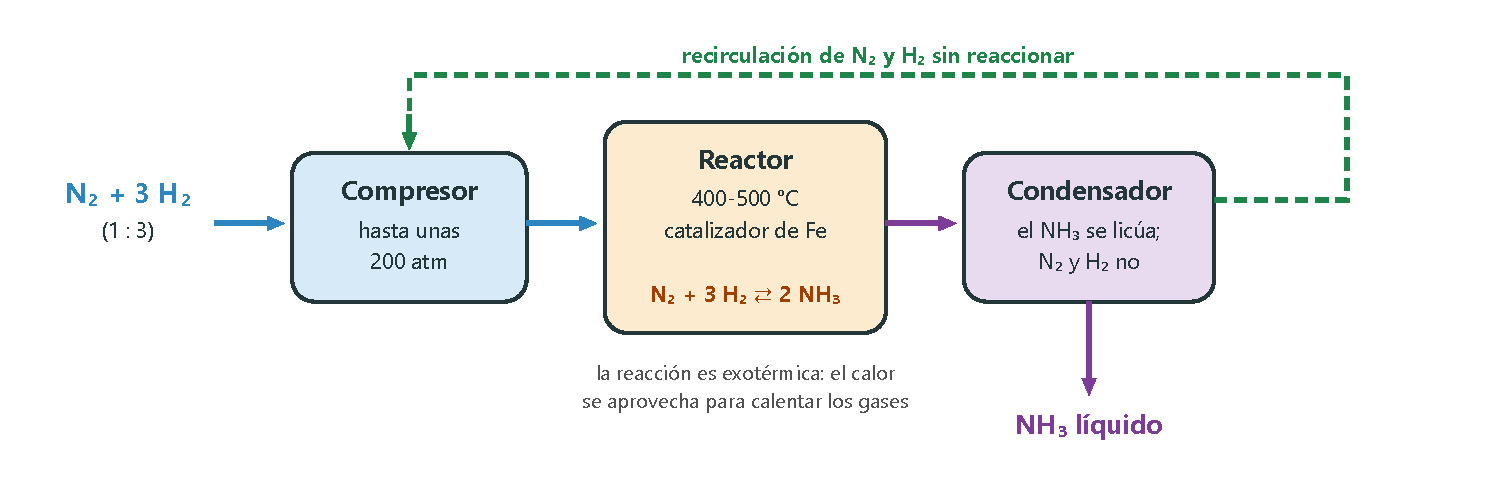
\includegraphics[width=0.85\textwidth]{images/UD6/haber_bosch}
    \caption{Esquema simplificado del proceso Haber-Bosch.}
    \label{fig:ud6-haber}
\end{figure}

\begin{exercise}
    En una planta de amoníaco se hacen reaccionar \qty{150}{\gram} de nitrógeno con \qty{30}{\gram} de hidrógeno. ¿Qué masa de
    amoníaco se obtiene si el rendimiento es del 60\,\%?
    \begin{solu}
        \textcolor{blue}{\(n(\ch{N2}) = 150/28 = \qty{5.36}{\mol}\), que necesitarían \qty{16.1}{\mol} de \ch{H2}; solo hay
        \(30/2 = \qty{15}{\mol}\): el \ch{H2} es el limitante. \(n(\ch{NH3}) = 15 \cdot \frac{2}{3} = \qty{10}{\mol}\) (\qty{170}{\gram}).}
        \(170 \cdot \num{0.60} = \textcolor{red}{\qty{102}{\gram}}\) de \ch{NH3}.
    \end{solu}
\end{exercise}

\begin{exercise}
    ¿Qué masa de amoníaco se obtiene, con un rendimiento del 60\,\%, si se mezclan \qty{3}{\litre} de \ch{H2} a \qty{2}{\atm} y
    \qty{4}{\litre} de \ch{N2} a \qty{1.8}{\atm}, ambos a \qty{25}{\degreeCelsius}?
    \begin{solu}
        \textcolor{blue}{\(n(\ch{H2}) = \dfrac{2 \cdot 3}{\num{0.082} \cdot 298} = \qty{0.246}{\mol}\);
        \(n(\ch{N2}) = \dfrac{\num{1.8} \cdot 4}{\num{0.082} \cdot 298} = \qty{0.295}{\mol}\). El \ch{H2} es el limitante (solo
        reacciona con \qty{0.082}{\mol} de \ch{N2}). \(n(\ch{NH3}) = \num{0.246} \cdot \frac{2}{3} = \qty{0.164}{\mol}\) (\qty{2.78}{\gram}).}
        \(\num{2.78} \cdot \num{0.60} = \textcolor{red}{\qty{1.67}{\gram}}\) de \ch{NH3}.
    \end{solu}
\end{exercise}

\subsection{La industria farmacéutica}

Desde la Antigüedad se han usado plantas para aliviar enfermedades: la adormidera como calmante, la manzanilla para el estómago…
A principios del siglo \textsc{xix}, con disolventes como el éter o el cloroformo, se aislaron los \textbf{principios activos} de
muchas de ellas, como la morfina o la cafeína, y en 1828 \textbf{Friedrich Wöhler} sintetizó en el laboratorio una sustancia
orgánica, la urea, a partir de compuestos inorgánicos. La \textbf{farmacología}, que estudia la composición, las propiedades y la
acción de los medicamentos, es una ciencia independiente desde mediados del siglo \textsc{xix}.

Desde que empieza la investigación hasta que un medicamento llega a la farmacia pueden pasar más de diez años:
\begin{enumerate}
    \item \textbf{Investigación y diseño}: se identifica la \textbf{diana} (normalmente una proteína relacionada con la enfermedad) y
    se busca un \textbf{principio activo} que actúe sobre ella. En la fase \textbf{preclínica} se estudia su seguridad y eficacia
    con modelos informáticos, en el laboratorio y en animales.
    \item \textbf{Ensayos clínicos}: se administra primero a un pequeño grupo de voluntarios sanos (fase I, seguridad y dosis),
    después a enfermos (fase II, eficacia) y finalmente en un estudio a gran escala (fase III).
    \item \textbf{Registro y comercialización}: las autoridades sanitarias evalúan los datos antes de autorizarlo. Una vez en el
    mercado, se sigue vigilando su seguridad (fase IV).
\end{enumerate}

\begin{remark}
    \textbf{Vacunas de ARN mensajero.} Las vacunas contra la COVID-19 se desarrollaron en un tiempo récord, pero gracias a décadas de
    investigación básica previa, como la de la bioquímica \textbf{Katalin Karikó} sobre el ARN mensajero, por la que recibió el
    premio Nobel en 2023. Como decía Ramón y Cajal: «Cultivemos la ciencia por sí misma, sin considerar por el momento las
    aplicaciones. Estas llegan siempre; a veces tardan años, a veces siglos».
\end{remark}

\subsection{Nuevos materiales}

La química, la física y la ingeniería de materiales desarrollan continuamente materiales con propiedades a la carta:
\begin{itemize}
    \item En \textbf{construcción}: madera translúcida, hormigón «autorreparable» con bacterias que sellan sus grietas o cementos
    que absorben luz de día y la emiten de noche.
    \item En \textbf{transporte}: espumas de aluminio, ligeras y resistentes a los impactos, o termoplásticos reciclables que
    aligeran coches y aviones y reducen su consumo.
    \item En \textbf{medicina}: prótesis de cerámica o de espuma de titanio, nanopartículas y liposomas que transportan fármacos
    hasta las células enfermas o materiales con memoria de forma.
    \item La \textbf{nanotecnología} manipula la materia átomo a átomo: a escala de nanómetros, los materiales presentan
    propiedades (resistencia, conductividad, reactividad) muy diferentes de las que tienen a mayor escala. El grafeno o los
    nanotubos de carbono son ejemplos.
\end{itemize}

\subsection{La química verde}

Durante mucho tiempo la industria química ha consumido grandes cantidades de recursos y ha emitido contaminantes al suelo, al aire
y al agua. La respuesta a este problema es la química verde.

\begin{definition}[Química verde o sostenible]
    Es una filosofía que busca diseñar productos y procesos químicos que reduzcan o eliminen el uso y la producción de sustancias
    peligrosas para la salud y el medio ambiente. Sus principios incluyen:
    \begin{itemize}
        \item \textbf{Prevenir} los residuos mejor que tratarlos después: procesos que incorporen al producto final todos los
        átomos de los reactivos (\textbf{economía atómica}).
        \item Usar y producir sustancias de \textbf{baja toxicidad} y minimizar el riesgo de accidentes.
        \item Ahorrar \textbf{energía} y usar fuentes y materias primas \textbf{renovables}.
        \item Usar \textbf{catalizadores} y diseñar productos \textbf{biodegradables}.
    \end{itemize}
\end{definition}

\begin{exercise}
    La economía atómica de un proceso es el porcentaje de la masa de los reactivos que acaba formando parte del producto deseado.
    Calcula la del proceso Haber-Bosch y la de la obtención de hidrógeno con zinc y ácido clorhídrico
    (\ch{Zn + 2 HCl -> ZnCl2 + H2}). ¿Cuál es más «verde» en este aspecto?
    \begin{solu}
        \textcolor{blue}{Haber-Bosch: todos los átomos acaban en el \ch{NH3}: \(\dfrac{34}{28 + 6} \cdot 100\).} \textcolor{red}{100\,\%}.
        \textcolor{blue}{Zinc: \(\dfrac{2}{\num{65.4} + 73} \cdot 100\).} \textcolor{red}{1,4\,\%}: casi toda la masa acaba en el
        subproducto, \ch{ZnCl2}. \textcolor{red}{El proceso Haber-Bosch es mucho más eficiente.}
    \end{solu}
\end{exercise}

\begin{exercise}
    Investiga sobre los diez medicamentos más vendidos en España: su principio activo, para qué se usan y alguna anécdota de su
    descubrimiento.
    \begin{solu}
        \textcolor{red}{Respuesta abierta.} Por ejemplo, el paracetamol y el ibuprofeno (analgésicos y antiinflamatorios), el
        omeprazol (protector gástrico), las estatinas (colesterol) o la amoxicilina (antibiótico, derivado de la penicilina
        descubierta por Fleming en 1928 al ver que un moho mataba sus cultivos de bacterias).
    \end{solu}
\end{exercise}

%========================================================================================
\section{Química en la vida: ¡al baño María!}\label{sec:ud6-bano}
%========================================================================================

Gracias a los programas de cocina, todo el mundo sabe lo que es cocinar al \textbf{baño María}: calentar un recipiente metiéndolo
en otro con agua caliente, en lugar de ponerlo directamente al fuego. El calor llega de forma lenta, suave y uniforme, y la
temperatura no pasa de \qty{100}{\degreeCelsius}, por lo que no se quema ni se altera lo que se calienta. Además de en la cocina, se
usa desde hace siglos en los laboratorios y en las industrias química, farmacéutica y cosmética.

Su origen nos lleva a la Alejandría del siglo \textsc{iii}, donde vivió \textbf{María la Judía}, una de las primeras alquimistas de
la historia, que lo utilizaba para destilar sustancias aromáticas y evaporar extractos. Sus obras se perdieron, quizá en el
incendio de la Biblioteca de Alejandría, pero las conocemos porque las citan otros autores, como su discípulo \textbf{Zósimo de
Panópolis}. Se le atribuyen también el \textit{tribikos}, un alambique de tres brazos para purificar sustancias por destilación, y
el \textit{kerotakis}, un aparato para extraer esencias de las plantas. Durante la Edad Media, muchos alquimistas usaron sus
técnicas en la búsqueda de la «quintaesencia», el supuesto quinto elemento, más puro que el agua, la tierra, el fuego y el aire.

Hoy sabemos que el agua es un medio excelente para calentar: tiene un \textbf{calor específico muy alto}
(\qty{4.18}{\joule\per\gram\per\degreeCelsius}) y, mientras hierve, su temperatura se mantiene constante.

\begin{exercise}
    a) ¿Por qué, al baño María, lo que se calienta no supera los \qty{100}{\degreeCelsius}? b) ¿Qué energía hace falta para calentar
    \qty{2}{\kilo\gram} de agua del baño de \qty{20}{\degreeCelsius} a \qty{90}{\degreeCelsius}? c) Elaborad en clase un
    \textbf{abecedario científico} con mujeres científicas destacadas de la historia; María la Judía puede ocupar la «J».
    \begin{solu}
        a) \textcolor{red}{Porque el agua líquida no puede superar su temperatura de ebullición} (a \qty{1}{\atm}): el calor
        adicional se emplea en evaporarla. b) \(Q = m\,c\,\Delta T = 2000 \cdot \num{4.18} \cdot 70 = \textcolor{red}{\qty{585}{\kilo\joule}}\).
        c) \textcolor{red}{Respuesta abierta}: por ejemplo, Hipatia, Marie Curie, Rosalind Franklin, Lise Meitner, Dorothy Hodgkin,
        Margarita Salas…
    \end{solu}
\end{exercise}

%========================================================================================
\section{Prácticas}\label{sec:ud6-practicas}
%========================================================================================

\subsection{Bicarbonato y vinagre: ¿quién es el reactivo limitante?}

\noindent\begin{minipage}[t]{0.48\textwidth}
    \textbf{Objetivo}
    \begin{itemize}
        \item Comprobar experimentalmente el concepto de reactivo limitante con la reacción del bicarbonato de sodio y el ácido
        acético del vinagre.
    \end{itemize}
\end{minipage}\hfill
\begin{minipage}[t]{0.48\textwidth}
    \textbf{Material y reactivos}
    \begin{itemize}
        \item Cinco botellas pequeñas de plástico iguales, cinco globos, embudo, probeta, balanza y cucharilla.
        \item Bicarbonato de sodio (\ch{NaHCO3}) y vinagre (ácido acético al 5\,\% en masa, \(d \approx \qty{1}{\gram\per\mL}\)).
    \end{itemize}
\end{minipage}

\textbf{Procedimiento}
\begin{enumerate}[label=\numberballgreen]
    \item Echa en cada botella \qty{50}{\mL} de vinagre.
    \item Con el embudo, pon en cada globo una cantidad distinta de bicarbonato: 1, 2, 3, 4 y \qty{6}{\gram}.
    \item Ajusta la boca de cada globo a una botella sin dejar caer el bicarbonato. Después, levanta los globos a la vez para que el
    bicarbonato caiga en el vinagre.
    \item Cuando acabe el burbujeo, compara el tamaño de los globos y observa si queda bicarbonato sin reaccionar en el fondo.
\end{enumerate}
\textbf{Trabaja con gafas.} La reacción es: \ch{NaHCO3(s) + CH3COOH(aq) -> CH3COONa(aq) + H2O(l) + CO2(g) ^}.

\begin{exercise}
    a) Calcula los moles de ácido acético que hay en \qty{50}{\mL} de vinagre y la masa de bicarbonato que reacciona exactamente con
    ellos. b) ¿En qué globos es limitante el bicarbonato y en cuáles el ácido? ¿Qué observarás? c) ¿Qué volumen de \ch{CO2} se
    obtiene como máximo a \qty{20}{\degreeCelsius} y \qty{1}{\atm}?
    \begin{solu}
        a) \textcolor{blue}{\(m(\text{ácido}) = 50 \cdot \num{0.05} = \qty{2.5}{\gram}\); \(n = \num{2.5}/60 = \qty{0.0417}{\mol}\).}
        \(m(\ch{NaHCO3}) = \num{0.0417} \cdot 84 = \textcolor{red}{\qty{3.5}{\gram}}\). b) \textcolor{red}{Con 1, 2 y \qty{3}{\gram}
        el limitante es el bicarbonato}: los globos crecen cada vez más y no sobra sólido. \textcolor{red}{Con 4 y \qty{6}{\gram}, el
        ácido}: los dos globos se inflan igual (el máximo) y queda bicarbonato en el fondo. c) \(V = \dfrac{\num{0.0417} \cdot
        \num{0.082} \cdot 293}{1} = \textcolor{red}{\qty{1.0}{\litre}}\).
    \end{solu}
\end{exercise}

\subsection{Química en la cocina: falso caviar de cacao}

\noindent\begin{minipage}[t]{0.48\textwidth}
    \textbf{Objetivo}
    \begin{itemize}
        \item Experimentar con una técnica de «cocina molecular», la gelificación en aceite frío, para obtener perlas parecidas al
        caviar.
    \end{itemize}
\end{minipage}\hfill
\begin{minipage}[t]{0.48\textwidth}
    \textbf{Material}
    \begin{itemize}
        \item \qty{30}{\gram} de cacao en polvo, \qty{50}{\gram} de azúcar, \qty{250}{\mL} de agua y \qty{2}{\gram} de agar-agar.
        \item Aceite de girasol, un vaso alto, un cazo, una jeringuilla grande y un colador.
    \end{itemize}
\end{minipage}

\textbf{Procedimiento}
\begin{enumerate}[label=\numberballgreen]
    \item Enfría el aceite en el vaso alto: en la nevera desde la noche anterior o media hora en el congelador. Debe estar a menos
    de \qty{4}{\degreeCelsius}.
    \item Mezcla en el cazo el cacao, el azúcar, el agua y el agar-agar y llévalo a ebullición, removiendo suavemente para no meter
    aire.
    \item Deja templar la mezcla al baño María (sin que llegue a cuajar) y carga la jeringuilla.
    \item Deja caer gotas en el aceite frío: al bajar, se enfrían y se convierten en perlas de gel que se depositan en el fondo.
    \item Cuela las perlas y acláralas con agua para quitarles el aceite.
\end{enumerate}
\textbf{Truco}: se puede sustituir el cacao por zumo de naranja, granadina o té matcha.

\begin{exercise}
    a) El agar-agar se disuelve en caliente (hacia \qty{90}{\degreeCelsius}) y gelifica al enfriarse (hacia \qty{40}{\degreeCelsius}),
    y el proceso se puede repetir. ¿Es un cambio químico o físico? b) ¿Por qué se usa aceite y no agua fría? c) Investiga qué es la
    esferificación con alginato y calcio, otra técnica de cocina molecular, y si es un proceso físico o químico.
    \begin{solu}
        a) \textcolor{red}{Físico}: es reversible y las moléculas del agar no cambian; solo forman una red que atrapa el agua al
        enfriarse. b) \textcolor{red}{Porque la mezcla es acuosa y no se mezcla con el aceite}: cada gota conserva su forma
        esférica mientras gelifica; en agua se disolvería. c) \textcolor{red}{Respuesta abierta}: el alginato de sodio (extraído
        de algas pardas) reacciona con los iones \ch{Ca^2+} y forma una membrana de alginato de calcio insoluble alrededor de la
        gota: es una \textcolor{red}{reacción química} (un intercambio de iones).
    \end{solu}
\end{exercise}

%========================================================================================
\section{Situación de aprendizaje: química verde (ODS 7, 12 y 13)}\label{sec:ud6-ods}
%========================================================================================

La industria química transforma materias primas en productos que mejoran nuestra vida y genera empleo y riqueza. Pero los
productos químicos liberados al medio ambiente han causado pérdida de biodiversidad, contaminación de aguas y suelos, el deterioro
de la capa de ozono o el aumento del efecto invernadero, además de consumir muchos recursos no renovables. La \textbf{química verde},
cuyas bases establecieron \textbf{Paul Anastas} y \textbf{John Warner} en 1998 con sus «doce principios», propone diseñar los
productos y los procesos para prevenir la contaminación desde el origen, durante todo su ciclo de vida.

Los \textbf{Objetivos de Desarrollo Sostenible 7} (energía asequible y no contaminante), \textbf{12} (producción y consumo
responsables) y \textbf{13} (acción por el clima) están muy relacionados con la industria química. La Unión Europea, a través del
\textbf{Pacto Verde Europeo}, se ha propuesto ser climáticamente neutra en 2050.

\begin{marker}
    \textbf{Reto:} elaborad un mural (físico o digital) con propuestas de la química verde que os parezcan más interesantes para
    reducir el impacto ambiental de la industria química, explicando a qué principios responden.
\end{marker}

\begin{enumerate}[label=\numberballred]
    \item \textbf{Investigad} los doce principios de la química verde y la trayectoria de sus «padres fundadores». Elegid un producto
    químico cotidiano (un detergente, un plástico, un fármaco) y analizad qué principios cumple o podría cumplir.
    \item \textbf{Investigad} un proceso industrial clásico, la obtención del ácido nítrico por el \textbf{método Ostwald}, cuyas
    etapas son:
    \ch{NH3 + O2 -> NO + H2O}; \ch{NO + O2 -> NO2}; \ch{NO2 + H2O -> HNO3 + NO}. ¿Qué residuos genera? ¿Cómo se
    aprovecha el \ch{NO} de la última etapa?
    \item \textbf{Calculad.} Ajustad las tres reacciones del método Ostwald. Si se parte de \qty{1000}{\litre} de amoníaco medidos
    en condiciones normales y el rendimiento global es del 85\,\%, ¿qué masa de ácido nítrico del 60\,\% en masa se obtiene?
    (Supón que el \ch{NO} de la tercera etapa no se recicla.)
    \item \textbf{Comunicad.} El mural debe incluir: los doce principios ilustrados con ejemplos; el análisis del producto elegido;
    el proceso Ostwald con sus impactos y alguna mejora sostenible, y una propuesta de consumo responsable para el día a día
    (reducir, reutilizar y reciclar; alimentación y movilidad sostenibles).
\end{enumerate}

\begin{exercise}
    Resuelve los cálculos del apartado 3 de la situación de aprendizaje.
    \begin{solu}
        \textcolor{blue}{Ajustadas: \ch{4 NH3 + 5 O2 -> 4 NO + 6 H2O}; \ch{2 NO + O2 -> 2 NO2};
        \ch{3 NO2 + H2O -> 2 HNO3 + NO}. Cada mol de \ch{NH3} da 1 mol de \ch{NO} y 1 de \ch{NO2}, y cada 3 de \ch{NO2} dan 2 de
        \ch{HNO3}: \(n(\ch{NH3}) = 1000/\num{22.4} = \qty{44.6}{\mol}\); \(n(\ch{HNO3}) = \num{44.6} \cdot \frac{2}{3} \cdot
        \num{0.85} = \qty{25.3}{\mol}\), es decir, \(\num{25.3} \cdot 63 = \qty{1594}{\gram}\) de \ch{HNO3} puro.}
        \(\dfrac{1594}{\num{0.60}} = \textcolor{red}{\qty{2.66}{\kilo\gram}}\) de ácido del 60\,\%.
    \end{solu}
\end{exercise}
